\newcommand{\DoNotLoadEpstopdf}{}
\pdfinfoomitdate=1
\pdftrailerid{}
\pdfsuppressptexinfo=15
\documentclass[11pt]{article}
\usepackage[letterpaper,margin=1in]{geometry}
\usepackage[T1]{fontenc}
\usepackage{lmodern}
\usepackage{amsmath,amssymb,amsthm,mathtools,amscd}
\usepackage{microtype}
\usepackage[dvipsnames]{xcolor}
\usepackage{graphicx,tikz}
\usetikzlibrary{arrows.meta,positioning,calc,fit,decorations.pathreplacing}
\usepackage{enumitem,needspace,booktabs,mathrsfs}
\usepackage[colorlinks=true,linkcolor=MidnightBlue,citecolor=MidnightBlue,urlcolor=MidnightBlue]{hyperref}
\hypersetup{pdftitle={Tame Hecke Eigensheaves with Several Marked Points},pdfauthor={OpenAI},pdfsubject={Constructible perverse eigensheaves for SL(n) with unipotent boundary monodromy},bookmarksdepth=2}
\newtheorem{theorem}{Theorem}[section]
\newtheorem{lemma}[theorem]{Lemma}
\newtheorem{proposition}[theorem]{Proposition}
\newtheorem{corollary}[theorem]{Corollary}
\newtheorem{claim}[theorem]{Claim}
\theoremstyle{definition}
\newtheorem{definition}[theorem]{Definition}
\theoremstyle{remark}
\newtheorem{remark}[theorem]{Remark}
\newcommand{\Gd}{\check G}
\newcommand{\cA}{\mathcal A}
\newcommand{\cB}{\mathcal B}
\newcommand{\cH}{\mathcal H}
\newcommand{\cO}{\mathcal O}
\newcommand{\cF}{\mathcal F}
\newcommand{\cL}{\mathcal L}
\newcommand{\cN}{\mathcal N}
\newcommand{\cS}{\mathcal S}
\newcommand{\Dlc}{D_{\mathrm{lcc}}}
\newcommand{\et}{\mathrm{et}}
\DeclareMathOperator{\Bun}{Bun}
\DeclareMathOperator{\Hecke}{Hecke}
\let\SS\relax
\DeclareMathOperator{\SS}{SS}
\DeclareMathOperator{\ad}{ad}
\DeclareMathOperator{\Lie}{Lie}
\DeclareMathOperator{\Res}{Res}
\DeclareMathOperator{\Spec}{Spec}
\DeclareMathOperator{\Rep}{Rep}
\DeclareMathOperator{\Perf}{Perf}
\DeclareMathOperator{\Loc}{Loc}
\DeclareMathOperator{\Gr}{Gr}
\DeclareMathOperator{\IC}{IC}
\DeclareMathOperator{\Hom}{Hom}
\DeclareMathOperator{\End}{End}
\DeclareMathOperator{\Aut}{Aut}
\DeclareMathOperator{\GL}{GL}
\DeclareMathOperator{\SL}{SL}
\DeclareMathOperator{\PGL}{PGL}
\DeclareMathOperator{\QCoh}{QCoh}
\DeclareMathOperator{\IndCoh}{IndCoh}
\DeclareMathOperator{\Nilp}{Nilp}
\DeclareMathOperator{\rk}{rk}
\DeclareMathOperator{\im}{im}
\DeclareMathOperator{\id}{id}
\DeclareMathOperator{\Tr}{Tr}
\DeclareMathOperator{\Perv}{Perv}
\DeclareMathOperator{\supp}{supp}
\numberwithin{equation}{section}
\setlist{itemsep=3pt,topsep=5pt}
\title{Tame Hecke Eigensheaves with Several Marked Points}
\author{OpenAI}
\date{October 5, 2026}
\begin{document}
\maketitle
\begin{abstract}
For $\SL_n$ in characteristic $p>n$, we construct nonzero locally constructible
perverse Hecke eigensheaves with Borel level at two or more marked points on a
smooth projective curve of genus at least two over an algebraic closure of a
finite field. The parameter is a Zariski-dense geometric $\ell$-adic
$\PGL_n$-local system with unipotent tame monodromy; its nilpotent logarithms
may have any Jordan type, including zero. The eigensheaves have parabolic
nilpotent singular support, and their eigenisomorphisms retain the full tensor
and fusion structure.
\end{abstract}
\setcounter{tocdepth}{1}
\tableofcontents
\clearpage
\section{Introduction}\label{intro:section}

A geometric Hecke eigensheaf realizes a local system on a curve through modifications of bundles. At a puncture, the monodromy of the local system must be reflected in the level structure on the bundle stack. We construct such eigensheaves for $\SL_n$ with Borel level at several punctures and arbitrary unipotent tame monodromy. The sheaves are locally constructible and perverse, and their eigenisomorphisms extend coherently over collisions of the modification points.

\subsection{The theorem}
Let $n\ge2$, let $k=\overline{\mathbb F}_q$ have characteristic $p>n$, and fix a prime $\ell\ne p$. Put $E=\overline{\mathbb Q}_\ell$. Let $X_0/\mathbb F_q$ be a smooth projective geometrically connected curve of genus $g\ge2$, with distinct rational points $x_1,\ldots,x_s$, where $s\ge2$. Write
\[
 X=(X_0)_k,\qquad D=x_1+\cdots+x_s,\qquad U=X\setminus|D|.
\]
Set $G=\SL_n$ and $\Gd=\PGL_{n,E}$, and let $B\subset G$ be the upper-triangular Borel subgroup. All bundle stacks below refer to the split group over the geometric base field in use.

A parameter is a continuous homomorphism
\begin{equation}\label{intro:parameter}
 \rho:\pi_1^{\et}(U,\bar u)\longrightarrow\PGL_n(L),
\end{equation}
where $L/\mathbb Q_\ell$ is finite inside $E$. We assume that its image is Zariski dense, that it kills wild inertia at every $x_i$, and that
\begin{equation}\label{intro:monodromy}
 \rho(\gamma)=\exp\bigl(t_{\ell,i}(\gamma)N_i\bigr)
 \qquad(\gamma\in I_{x_i}).
\end{equation}
Here $t_{\ell,i}:I_{x_i}\to\mathbb Z_\ell$ is a chosen tame quotient and $N_i\in\mathfrak{pgl}_n(L)$ is nilpotent. The exponential is the finite nilpotent exponential. No regularity is assumed for $N_i$; it may be zero. For $V\in\Rep_E(\Gd)$, write $V_\rho$ for the corresponding lisse $E$-sheaf on $U$.

Let
\[
 \cA=\Bun_{\SL_n,B,D}(X)
\]
be the stack of $\SL_n$-bundles $P$ together with Borel reductions $\beta_i$ at the marked points. A geometric $E$-adic complex $M$ on $\cA$ is \emph{locally constructible perverse} if $f^*M[d]$ is bounded constructible and perverse for every smooth finite-type chart $f:S\to\cA$ of constant relative dimension $d$. This is a local condition on the stack.

The trace pairing identifies its cotangent vectors with Higgs fields
\begin{equation}\label{intro:cotangent}
 \phi\in H^0\bigl(X,\ad(P)\otimes\omega_X(D)\bigr),
 \qquad \Res_{x_i}(\phi)\in\Lie R_u(B_{\beta_i})
 \quad(1\le i\le s).
\end{equation}
Let $\Lambda_D$ be the cone of these fields that are nilpotent at the generic point of $X$. A singular-support containment in this cone means its smooth cotangent pullback on every smooth chart.

For a finite set $I$ and representations $V_i\in\Rep_E(\Gd)$, the functor $\Hecke_{I,(V_i)}$ modifies bundles at points of $U^I$. We use relative Satake normalization: on a Schubert cell of dimension $d_\lambda$ the kernel is $E[d_\lambda](d_\lambda/2)$, and there is no additional moving-leg shift. The conventions and collision maps are specified in Section~\ref{found:section}.

\Needspace{12\baselineskip}
\begin{theorem}\label{intro:main}
For every parameter \eqref{intro:parameter} satisfying the preceding hypotheses, there is a nonzero locally constructible perverse geometric $E$-adic sheaf $M$ on $\cA$ with
\[
 \SS(M)\subset\Lambda_D.
\]
For every finite set $I$ and every family $(V_i)_{i\in I}$, it has isomorphisms
\begin{equation}\label{intro:eigen}
 \Hecke_{I,(V_i)}(M)
 \simeq M\boxtimes\Bigl(\mathop{\boxtimes}_{i\in I}(V_i)_\rho\Bigr)
 \qquad\text{on }\cA\times U^I,
\end{equation}
natural in the representations and coherent for the tensor unit, convolution, permutations, and fusion on every collision diagonal. These isomorphisms use the relative normalization above.
\end{theorem}

The parameter and eigensheaf are geometric: the statement does not require a Frobenius structure. Local constructibility allows the cohomological bounds to depend on the finite-type chart.

\subsection{Context and antecedents}
The eigensheaf problem originates in Drinfeld's rank-two construction and
Laumon's geometric formulation for general linear groups
\cite{Drinfeld,Laumon}. Frenkel, Gaitsgory, and Vilonen reduced unramified
$\GL_n$ eigensheaf existence to a vanishing conjecture \cite{FGV}, which
Gaitsgory subsequently proved \cite{GaitsgoryVanishing}. Geometric Satake
identifies the local Hecke kernels with representations of the dual group
and supplies their tensor and fusion structure \cite{MV}. These results
established the geometric form of the passage from a prescribed local
system to an automorphic sheaf.

Our immediate antecedent is \cite[Theorem~1.1]{CT}, whose main theorem
has one marked point and regular-unipotent monodromy for a broader class
of groups. Here the group is $\SL_n$ with $p>n$, there are several marked
points, and every nilpotent boundary logarithm is allowed. The
two-specialization construction and the local arguments follow that
companion; we prove the simultaneous level geometry and compatibility
arguments needed for this extension.

For semisimple groups over $\mathbb C$, Beilinson and Drinfeld constructed
eigensheaves from opers by quantizing the Hitchin system \cite[\S0.2]{BD}.
The recent five-paper collaboration proves categorical forms of the
unramified correspondence in characteristic zero \cite{GLCI,GLCV}.
Arinkin, Gaitsgory, Kazhdan, Raskin, Rozenblyum, and Varshavsky introduced
the stack of local systems with restricted variation and its action on
sheaves with nilpotent singular support \cite{AGKRRV}.
Gaitsgory and Raskin use this framework to formulate the geometric adic
correspondence and compare characteristic zero with positive characteristic
\cite{GR}. The input needed here is the characteristic-zero restricted
equivalence \cite[Main Theorem~1.3.9(ii)]{GR}, through the unramified
eigencomplex construction of \cite[Lemma~8.1]{CT}. Thus the categorical
theory enters on a smooth projective curve before level structures are
introduced.

Nilpotent singular support links this input to ramification. The geometry
of the global nilpotent cone was developed by Laumon, Faltings, and Ginzburg
\cite{LaumonNilpotent,Faltings,GinzburgNilpotent}. Beilinson's theory of
singular support for constructible \'etale sheaves, and Barrett's extension
to adic coefficients, give the function tests used below
\cite{Beilinson,Barrett}. The Hecke detection argument in
\cite[\S\S20.5--20.8, Appendix~H]{AGKRRV} uses a cocharacter in the center
of a Levi subgroup and an isolated cotangent intersection. The field and
specialization arguments of \cite[\S\S3--4]{CT} adapt that geometry. We establish
the versions required for all the level stacks occurring here.
Geometric nearby cycles and their perverse exactness rest on
Hansen--Scholze and Gaitsgory--Raskin \cite{HS,GR}.

The characteristic-zero level arguments use Betti sheaf theory.
Nadler and Yun prove local constancy of moving Hecke operators on the
nilpotent category and construct its spectral action, already allowing
finitely many level points \cite[Theorems~6.2.2 and~6.3.7]{NY}.
Their automorphic gluing construction relates twisted nodal curves to
smoothings \cite{NYGluing}; its description of bundle types and branch
gluing is the geometric antecedent of our degeneration. Our proof also
needs a separate nonvanishing statement for the particular nearby cycles
being taken. At a puncture, the local spectral input comes from
Gaitsgory's central sheaves \cite{GaitsgoryCentral}, the affine-flag
equivalence of Arkhipov and Bezrukavnikov \cite{AB}, and Dhillon and
Taylor's extension to the universal monodromic setting \cite{DT}.
The last supplies the local kernels used in the descent argument of
\cite[\S7]{CT}, which we globalize with all the other levels retained.
Dhillon and Taylor's sequel proves the tame local Betti correspondence
\cite{DTLocal}.

Several-point ramification has earlier geometric realizations. Uit de Bos
gives an explicit $\GL_2$ correspondence for the projective line with four
punctures and pure irreducible parameters with unipotent monodromy
\cite{UitDeBos}. Shen proves a Hecke-compatible equivalence over an open
spectral locus for parabolic $\GL_n$ in positive characteristic, using
crystalline $D$-modules \cite{Shen}. In the characteristic-zero de Rham
setting, F{\ae}rgeman gives a construction for irreducible regular-singular
parameters conditional on the forthcoming factorization input and local
compatibility conjecture specified in that work
\cite[Theorem~1.4.1.1, \S\S1.3.7, 1.4.3, Conjecture~4.2.1]{Faergeman}.
In the cited version,
regular holonomicity and generic perversity in the ramified setting are
stated as expectations \cite[Remark~1.4.1.2]{Faergeman}. The present
theorem concerns geometric adic sheaves in positive characteristic and
includes local constructibility and perversity.


\subsection{Proof strategy and the several-point extensions}
The proof has two specializations. First we construct an eigensheaf with the prescribed level in characteristic zero. We then specialize it to the given curve in characteristic $p$. The intermediate sheaves must remain locally constructible, retain the full Hecke system, and remain nonzero. The last condition requires a separate argument: nearby cycles of a nonzero complex can vanish.

The first stage starts with any marked complex curve and a dense parameter with unipotent boundary monodromy. Take two copies of that curve and join corresponding marked points to form a nodal curve. A smoothing replaces all its nodes at once. On the second component, reverse the orientation of the underlying marked surface and transport the parameter. This makes the two boundary monodromies inverse at every pair of branches. Finite quotients of the parameter then glue at all nodes after introducing suitable cyclic stabilizers there. Their compatible lifts produce a dense unramified parameter on the smooth geometric generic curve, where the characteristic-zero existence theorem applies.

The cyclic stabilizer type of the bundles has a different role from the boundary monodromy of the parameter. Choosing that type inside an alcove turns the special bundle stack into a quotient of two stacks with \emph{enhanced flags}. An enhanced flag is a reduction to $N_B=R_u(B)$; forgetting it is a torsor under $T=B/N_B$. With $s$ nodes, the special stack is
\[
 \bigl[(\cA_1^+\times\cA_2^+)/T^s\bigr],
\]
where the torus changes the two branch enhancements at each node simultaneously. All node identifications must be compatible with the same parameter tower. One second component suffices: the extra cycles in the dual graph give gluing choices and impose no further relation between the nodes.

After nearby cycles, pull back to the product and restrict to a fiber over the second factor. This gives an eigencomplex on the first enhanced stack. To pass to ordinary flags, we prove that its monodromies along the enhancement torus are unipotent. The local central-kernel trace at a puncture identifies representation characters of that torus monodromy with traces of the parameter's boundary monodromy. The latter traces are $\dim V$, for every $V$, under \eqref{intro:monodromy}. Characters therefore force all enhancement eigencharacters to be trivial. Compactly supported cohomology along the torus is then nonzero, so forgetting the enhancements preserves a nonzero eigencomplex. This is the step where unipotence, rather than regular unipotence, is sufficient.

Two further arguments control the sheaves throughout. A local calculation with two Hecke modifications detects covectors outside the nilpotent cone. The same calculation, applied to cuts over a trait, proves that nearby cycles cannot vanish when the closure of the nonzero generic stalks meets the special fiber. Separately, the Betti spectral action makes fixed-point Hecke functors exact near a dense parameter: an equivariant frame near its free closed orbit identifies these functors with finite sums of the identity. Moving-leg local constancy then permits perverse cohomology while retaining every tensor and collision comparison.

To reach the given curve, lift it with its marked points over the Witt ring $W(k)$. The finite quotients of $\rho$ extend over root stacks at the marked sections, whose orders are powers of $\ell$. Proper henselian lifting gives a compatible parameter on the geometric generic curve with the same dense image and boundary monodromies. Apply the characteristic-zero construction to that parameter and take geometric nearby cycles on the ordinary Borel-level bundle stack. Proper bounded Hecke modifications make the closure of the nonzero generic-stalk locus meet the special fiber, allowing the detection criterion to prove nonvanishing once more.

These constructions extend the one-point argument of \cite{CT}. The additional work is to prove the detection and perverse statements for the several-level stacks, to keep the other levels transported in the local central-kernel comparison, and to glue one compatible tower at all nodes. The detection criterion and the torus descent are stated separately from the final construction, so their hypotheses and their use in both specializations remain explicit. The nearby-cycle and unramified existence inputs are recalled with their precise scope; the several-point extensions are proved here.

Section~\ref{found:section} fixes the sheaf and Hecke conventions. Section~\ref{geom:section} proves the cotangent and transverse-modification facts used in the detection theorems of Section~\ref{det:section}. Sections~\ref{perv:section} and~\ref{desc:section} establish perverse cohomology and descent from enhanced flags. Section~\ref{con:section} carries out the characteristic-zero construction, and Section~\ref{lift:section} specializes it to prove Theorem~\ref{intro:main}.

\section{Level structures, sheaves, and specialization}
\label{found:section}

The construction will pass through enhanced flags and through a quotient
that identifies paired enhancements on two marked curves.  We describe these stacks
first, then fix the sheaf and Hecke conventions that allow the resulting
objects to be specialized.  The nearby-cycle inputs are
\cite[Propositions~2.1 and~5.1]{CT}; their hypotheses concern the local
geometry at the moving legs, rather than the number of level points.

\subsection{The level stacks}
\label{found:level-stacks}

Let $X$ be a smooth projective connected curve over an algebraically
closed field, and let $D=x_1+\cdots+x_s$ be a reduced divisor.  Write
$U=X\setminus |D|$.  We use $G=\mathrm{SL}_n$, the upper triangular
Borel $B$, its unipotent radical $N_B$, and the diagonal torus
$T=B/N_B$.  The stacks
\[
 \cA=\Bun_{G,B,D}(X),\qquad
 \cA^+=\Bun_{G,N_B,D}(X)
\]
classify a $G$-bundle with, respectively, a $B$-reduction or an
$N_B$-reduction at every $x_i$.  We call the latter an enhanced flag.
Forgetting the enhancements gives a representable torsor
\begin{equation}\label{found:torsor}
                         q:\cA^+\longrightarrow\cA
                         \quad\text{under }T^s.
\end{equation}
Unlevelled bundles and opposite Borels are also allowed.  All these
stacks are smooth and locally of finite type: the bundle deformation
obstruction lies in $H^2$ on a curve, and adding a reduction at a point
has smooth fiber $G/B$ or $G/N_B$.

For two such pointed curves, identify the flag tori at corresponding
points by fixed isomorphisms $\tau_i:T_{1i}\simeq T_{2i}$.  Put
\begin{equation}\label{found:quotient}
 \cB_{12}=[(\cA_1^+\times\cA_2^+)/T^s_\Delta],\qquad
 T^s_\Delta=\prod_{i=1}^s\{(t,\tau_i(t)):t\in T_{1i}\}.
\end{equation}
The branch convention in the nodal construction will specify the
$\tau_i$.  This smooth stack maps to $\cA_1\times\cA_2$ as a torsor
under $(T_1^s\times T_2^s)/T^s_\Delta$.  We will use this quotient in
characteristic zero.  Thus its objects are pairs of enhanced bundles
modulo simultaneous changes of the two enhancements at each paired
marking.

A Hecke modification in $U$ transports every level structure, because
it identifies the bundles near all the $x_i$.  On the product and the
quotient, a leg in $U_1\sqcup U_2$ modifies the corresponding component.
The quotient Hecke correspondence pulls back to the product
correspondence when either its input or its output is lifted to the
product.  Indeed the transported enhancements provide the lift on the
other side.  This cartesian property also holds for successive
modifications and their collision diagrams.

On a fixed Schubert bound, both the input-and-leg and output-and-leg
maps are representable and proper.  On an exact-position stratum they
are smooth.  To see that adding all the levels preserves these facts,
choose a coordinate and a frame on the formal disc at the leg.  The
modification is a split affine-Grassmannian model there; the marked
fibers remain in the complementary piece of the gluing.  For a fixed
bound the frame can be taken to finite jet order, so these descriptions
are obtained by smooth covers.  The same description applies to a leg
in the smooth scheme locus of a family of twisted nodal curves.  Its
stacky nodes remain in the complementary piece.  Restricting to fixed
node types restricts both bounded projections by base change and hence
preserves their properness.  On a finite-type output chart a fixed
bound meets only a quasi-compact part of the input stack.

\subsection{Local constructibility and relative Satake}

Put $E=\overline{\mathbb Q}_\ell$.  For a smooth stack $\cB$ locally of
finite type, $\Dlc(\cB,E)$ denotes the geometric adic complexes whose
ordinary pullback to every smooth finite-type scheme chart is bounded
constructible.  Thus ``lcc'' means locally bounded constructible, and
bounds may depend on the chart.  An object $F$ is perverse when
$f^*F[d]$ is perverse for every smooth chart $f:S\to\cB$ of constant
relative dimension $d$.  These conditions define a perverse
$t$-structure and its truncations locally on the stack.

For a closed conic subset $C\subset T^*\cB$, set
\[
 f^\circ C=\operatorname{image}
   (S\times_{\cB}C\longrightarrow T^*S).
\]
The assertion $\SS(F)\subset C$ means
$\SS(f^*F)\subset f^\circ C$ on every such chart.  Here stack
cotangent vectors mean degree-zero cotangent vectors, and singular
support is the geometric adic singular support, with the
function-test characterization of \cite[\S1.5, Theorem~(vii)]{Barrett}.
Shifts do not affect singular support.

Fix a Satake equivalence with $\Rep_E(\Gd)$, where $\Gd=\mathrm{PGL}_n$,
including its fusion commutativity constraint.  Write $\rho_G$ for the
half-sum of positive roots.  For a dominant
coweight $\lambda$ its simple kernel has open-orbit restriction
\begin{equation}\label{found:satake-normalization}
 \IC_\lambda|_{\Gr^\lambda}
       =E[d_\lambda](d_\lambda/2),\qquad
 d_\lambda=\langle 2\rho_G,\lambda\rangle.
\end{equation}
The integer $d_\lambda$ is even: the coweight lattice of $\mathrm{SL}_n$
is the coroot lattice, and $\langle2\rho_G,\alpha^\vee\rangle=2$ for a
simple coroot.  Tate twists here are geometric coefficient lines;
compatible trivializations may be chosen for Betti comparison.

For a finite set $I$ let $\cH_I$ be the moving Hecke stack, with input
map $p_I$ and output-and-leg map $o_I:\cH_I\to\cB\times U^I$.
The relative Satake kernel $\operatorname{Sat}_I(\boldsymbol V)$ for
$\boldsymbol V=(V_i)_{i\in I}$ is the exterior product of the
fixed-point kernels at distinct legs, extended by fusion at collisions.
Equivalently, it is computed using successive modifications and proper
convolution.  We define
\begin{equation}\label{found:hecke}
 \Hecke_{I,\boldsymbol V}(F)
   =o_{I,*}\bigl(F\,\widetilde\boxtimes\,
                         \operatorname{Sat}_I(\boldsymbol V)\bigr).
\end{equation}
In input frames the twisted product is the ordinary exterior product;
Satake equivariance supplies descent.  The push is taken on a finite
bound containing the kernel support.  There is no moving-leg shift in
\eqref{found:hecke}; in particular
$\Hecke_{I,(\mathbf1)}(F)=F\boxtimes E_{U^I}$.

\begin{definition}\label{found:coherence}
A coherent eigenstructure for a tensor local system
$V\mapsto L_V$ on $U$ consists of natural isomorphisms
\[
 \Hecke_{I,\boldsymbol V}(F)
       \simeq F\boxtimes\Bigl(\mathop{\boxtimes}_{i\in I}L_{V_i}\Bigr)
\]
for all finite sets and representations, compatible with the unit,
successive modifications and convolution, permutations, and fusion.
Explicitly, if $a:I\twoheadrightarrow J$ and
$\delta_a:U^J\to U^I$ is its collision diagonal, the fusion comparison
uses ordinary pullback and identifies
\[
 (1\times\delta_a)^*\Hecke_{I,\boldsymbol V}(F)
 \simeq\Hecke_{J,\boldsymbol W}(F),\qquad
 W_j=\bigotimes_{i\in a^{-1}(j)}V_i.
\]
The eigenmaps must commute with these comparisons, including their
compositions for nested collisions.
\end{definition}

We use this convention for products and quotients as well, allowing
legs on both component curves.  When studying perversity over $U^I$
we will insert $[|I|]$ explicitly and subsequently remove it.

\subsection{Geometric nearby cycles}

Let $R$ be an excellent complete strictly henselian discrete valuation
ring with algebraically closed residue field and with $\ell$ invertible.
Write $S=\Spec R$, fix a geometric generic point $\bar\eta$, and write
$0$ for the closed point.  Geometric nearby cycles
$\Psi_Y:D^b_c(Y_{\bar\eta},E)\to D^b_c(Y_0,E)$ take no inertia
invariants.  If descent data supply an inertia action, we use the
underlying geometric complex.

\begin{proposition}[Nearby-cycle input]\label{found:nearby}
For finite-type $S$-schemes, geometric nearby cycles preserve bounded
constructibility, are perverse exact, commute with smooth pullback and
proper pushforward, and satisfy exterior-product comparison.  They are
unchanged by finite extensions of the trait inside the fixed geometric
generic field.  The same statements hold locally on the smooth stacks
used here, with representable proper maps.

Let $Z$ be a finite-type $S$-scheme.  Suppose a lisse finite-rank sheaf
$L_{\bar\eta}$ on $Z_{\bar\eta}$ has
a lattice over the integers of a finite extension of $\mathbb Q_\ell$.
Assume that each finite reduction extends lisse over $Z$ after a finite
extension of $S$, compatibly on further common extensions, with special
reductions belonging to a fixed lisse sheaf $L_0$ on $Z_0$.  The trait
extension may depend on the reduction.  Then for any map $g:Y\to Z$
of finite-type $S$-schemes and any bounded constructible $F$ on $Y_{\bar\eta}$,
\begin{equation}\label{found:lattice}
 \Psi_YF\otimes g_0^*L_0
      \xrightarrow{\sim}
       \Psi_Y(F\otimes g_{\bar\eta}^*L_{\bar\eta}).
\end{equation}
This is natural in maps and tensor products of the lisse systems, and
holds locally on the smooth stacks in use.
\end{proposition}

These are precisely the assertions of \cite[Proposition~2.1]{CT}.
We recall why they apply to geometric coefficients without a common
finite field of descent.  At a fixed torsion coefficient level, each
finite diagram descends after a finite trait extension.  The comparisons
are compatible with further extensions and with reduction of the
coefficients.  Passing to the adic system, then inverting the coefficient
uniformizer, gives the geometric functor.  Equivalently, over the
integral closure of $R$ in its geometric generic field, the universally
locally acyclic extension formalism gives nearby cycles by special
restriction; see \cite[Theorems~4.1 and~6.7]{HS}.  Smooth descent gives
the stack assertions, including perversity with the chart shift $[d]$.
For \eqref{found:lattice}, apply the lisse tensor formula to each
extended finite reduction and pass to the limit.  This permits arbitrary
$g$: it is the lisseness of the factor, rather than a base-change claim
for $\Psi$ along $g$, that is used.  No single finite extension is
required for the entire lattice tower.

All these comparisons use the natural pull, tensor, and proper-push
exchange maps.  They respect composition, tensor associativity,
projection formula, and proper base change.  We will also use the
constant-family property: a complex pulled back from a fixed geometric
fiber has zero vanishing cycles in a smooth constant family.

\begin{proposition}[Specialization of eigenstructures]
\label{found:hecke-specialization}
Let $\cB/S$ be smooth and locally of finite type, and let
$\mathscr U/S$ be a smooth curve of allowed legs.  Assume the split
spherical disc models, proper bounds, and smooth exact-position maps
described in Section~\ref{found:level-stacks}.  Then there are natural
comparisons
\[
 \Hecke^0_{I,\boldsymbol V}(\Psi F)
   \xrightarrow{\sim}
 \Psi_{\cB\times_S\mathscr U^I}
             \Hecke^{\bar\eta}_{I,\boldsymbol V}(F)
 \qquad(F\in\Dlc(\cB_{\bar\eta},E)),
\]
compatible with the entire relative Hecke system of
Definition~\ref{found:coherence}.  Consequently, if $F$ has a coherent
lisse eigenvalue whose lattices satisfy Proposition~\ref{found:nearby}
compatibly as a tensor system, $\Psi F$ has the specialized coherent
eigenvalue.
\end{proposition}

\begin{proof}
This is \cite[Proposition~5.1]{CT}; we explain the local hypothesis and
the collision assertion needed here.  In a coordinate-and-input-frame
cover a bounded step is a product with a split Schubert model.  For an
arbitrary preceding space $Y$ and a complex $K$ on it, the comparison
for the next twisted product is therefore the exterior-product map
\[
 \Psi_YK\boxtimes\Psi_{\Gr}\operatorname{Sat}(V)
 \xrightarrow{\sim}
 \Psi_{Y\times_S\Gr}(K\boxtimes\operatorname{Sat}(V)).
\]
The first factor need not be smooth.  The specialized Grassmannian
kernel is the Satake kernel with the same label and normalization;
\cite[Lemma~5.3]{CT} fixes a single tensor identification for these
kernels.  Frame descent and proper push give the one-step comparison.

For successive steps, take $Y$ to retain the preceding modifications
and all leg parameters.  The same calculation is valid after setting
any collection of legs equal.  Proper convolution then gives the fused
comparison, and naturality of the exchange maps identifies it with the
comparison obtained by successive pushes.  Thus the diagonal exchange,
which need not be invertible on arbitrary sheaves, is invertible on
these Hecke constructions and respects nested diagonals.  Permutations
are the fusion symmetry of the kernels, and the identity-modification
kernel gives the unit.  Transported levels at all marked points, and
node types away from the disc, change none of these frame calculations.
This verifies the application of the cited proposition to every stack
and family used here.  Finally \eqref{found:lattice} identifies the
specialization of the eigenvalue side, naturally in all its tensor
maps, and hence specializes the coherence diagrams themselves.
\end{proof}

\subsection{Betti comparison}
\label{found:betti}

Over $\mathbb C$ we use the realization of geometric adic constructible
complexes as algebraically constructible complexes of ordinary
$E$-vector spaces on the analytic space.  For a lisse sheaf it restricts
its continuous monodromy to topological loops.  On finite-type charts
it is conservative, preserves perversity, and commutes with the
pullbacks, tensor products, and finite-type pushes used below.  It also
identifies algebraic singular support with the complex conic analytic
singular support, as seen from comparison of vanishing-cycle tests.
These conventions and their passage to smooth stacks are those of
\cite[\S2.4]{CT}; see also \cite[\S2.2.1]{GR}.

We use Betti results to verify properties of already constructed adic
objects and adic comparison maps.  In particular, Betti perversity
bounds will justify adic truncation comparisons.  The infinite-rank
universal monodromic kernels used in the torus argument stay on the
Betti side.  Every object subsequently specialized is geometric adic
and lcc.

\section{Nilpotent covectors and transverse Hecke modifications}
\label{geom:section}

The sheaf-theoretic detection argument needs two geometric inputs: a
dimension bound for the nilpotent cotangent cone and a transverse Hecke
modification for every covector outside it.  We prove these for all the
level stacks of Section~\ref{found:level-stacks}.  Throughout this
section the ground field $\Bbbk$ is algebraically closed of characteristic zero
or of characteristic $p>n$; the product and quotient stacks are needed
only in characteristic zero.  Put $\mathfrak g=\Lie G$, and write
$\mathfrak m=\Lie M$ for a Levi subgroup $M$.

\subsection{The matrix hypotheses and the cotangent cone}

The trace form $\kappa(a,b)=\operatorname{tr}(ab)$ is nondegenerate on
$\mathfrak{sl}_n$, since $n$ is invertible.  We record the other Lie
algebra facts that underlie \cite[\S3]{CT}, with the characteristic
hypotheses checked for our group.  A Levi has block sizes
$d_1,\ldots,d_r$ with sum $n$.  Its Lie center consists of block scalars
$(c_i)$ with $\sum_i d_ic_i=0$.  The trace form there is the restriction
of $\sum_i d_ic_ic'_i$.  Each $d_i$ and $n$ is invertible, so this
restriction is nondegenerate: its orthogonal complement in the block
scalar space is the line $(1,\ldots,1)$, whose norm is $n$.

Chevalley restriction for such a Levi follows from the characteristic
polynomials of the blocks.  The Levi Weyl group has order
$\prod_i d_i!$ invertible in the field, so restriction to the trace-zero
hyperplane commutes with taking invariants.  Symmetric polynomials in
the block eigenvalues give all invariants there; injectivity follows
from the density of matrices with distinct eigenvalues within the
blocks.  Conjugators may be chosen with determinant one by adjusting
a diagonal centralizer element.  The scheme centralizer of a semisimple
matrix is the corresponding block Levi.  Finally, matrix nilpotence
agrees with the zero fiber of these invariants, and every nilpotent
matrix over \emph{any} field extension has a rational full flag on
which it is strictly triangular.  Such a flag is obtained successively
from nonzero vectors in the kernel and the induced nilpotent operator
on the quotient.  These verify the four group hypotheses used in
\cite[\S\S1 and~3]{CT}, without extending the field to find a nilpotent
flag.

Let $P$ be a bundle with reductions $H_i$ at $x_i$, where each $H_i$
is a Borel or its unipotent radical.  Its deformation bundle is
\[
 \mathcal E_H=\ker\left(\ad(P)\longrightarrow
              \bigoplus_i\ad(P)_{x_i}/\mathfrak h_i\right),
 \qquad \mathfrak h_i=\Lie H_i.
\]
Infinitesimal automorphisms and deformations are $H^0(\mathcal E_H)$
and $H^1(\mathcal E_H)$.  Serre duality identifies degree-zero
cotangent vectors with Higgs fields
\begin{equation}\label{geom:residues}
 \phi\in H^0(X,\ad(P)\otimes\omega_X(D)),\qquad
            \Res_{x_i}\phi\in\mathfrak h_i^\perp.
\end{equation}
The trace form gives
$\mathfrak b_i^\perp=\Lie N_{B_i}$ and
$(\Lie N_{B_i})^\perp=\mathfrak b_i$.  Thus ordinary flags impose
nilradical residues, whereas enhanced flags impose Borel-valued
residues.  For unlevelled bundles the fields are regular.

On $\cB_{12}$ a cotangent vector pulls back to a pair of enhanced-level
fields that annihilates the diagonal torus action.  Pairing a covector
with an infinitesimal change of enhancement is pairing with the toral
part of its residue.  The two branch contributions are added with the
signs fixed by the identifications $\tau_i$ in
\eqref{found:quotient}.

\begin{definition}\label{geom:cone}
For any of these stacks $\cB$, let $\Lambda\subset T^*\cB$ be the cone
of Higgs fields generically nilpotent on each component curve in its
presentation.  For a smooth chart $f:S\to\cB$, write
$\Lambda_S=f^\circ\Lambda$.
\end{definition}

The cone is closed, since the nonleading coefficients of the
characteristic polynomial are global sections whose vanishing is
exactly generic nilpotence.  Its enhanced-level residues have zero
toral part.  Indeed, writing $\phi=b(t)\,dt/t$ at a marked point,
the characteristic coefficients of $b(t)$ vanish and hence those of
$b(0)$ vanish.  A nilpotent upper triangular matrix has zero diagonal.
Consequently the enhanced cone is precisely the smooth cotangent
pullback of the ordinary cone under $q$.  Likewise, the cone on
$\cB_{12}$ is the smooth cotangent pullback from
$\cA_1\times\cA_2$.  All toral residues vanish already, so the
quotient imposes no additional condition on this cone.

\begin{proposition}\label{geom:dimension}
For a smooth finite-type chart $S\to\cB$ of pure dimension $d$,
\[
                            \dim\Lambda_S\le d.
\]
In characteristic zero the cone is isotropic: the symplectic form
vanishes on the smooth locus of every reduced subvariety of
$\Lambda_S$.
\end{proposition}

\begin{proof}
We adapt the rational-reduction proof of \cite[Proposition~3.1]{CT}
to all the marked flags.  This is the parabolic form of Ginzburg's
isotropy argument \cite[Lemma~7]{GinzburgNilpotent}; compare the
separable-lifting criterion and its bundle-stack application in
\cite[Appendix~D.1.5 and~D.1.8]{AGKRRV}.  For $\mathrm{SL}_n$ the
required flag is already rational.  First take ordinary flags, and let $Z$ be a
reduced irreducible component of $\Lambda_S$, with function field $F$.
Its generic point supplies $(P,(\beta_i),\phi)$ on $X_F$, together
with its lift to $S$.  Over $F(X)$, choose a rational full flag in the
underlying rank-$n$ vector space that makes the nilpotent field strictly
triangular.  Properness of the associated flag bundle extends this
Borel reduction to the whole smooth curve $X_F$.  Denote it by $Q$.
Its nilradical bundle is a subbundle of $\ad(P)$, so generic
containment extends to
\[
 \phi\in H^0\bigl(X_F,
       (Q\times^B\Lie N_B)\otimes\omega_{X_F}(D)\bigr).
\]
No separable or inseparable extension of $F$ has been used.

For each $i$, fix the relative position of $Q_{x_i}$ and $\beta_i$.
Let $\mathcal Y$ classify a global Borel reduction and flags with
these prescribed relative positions.  This is a smooth stack:
$\Bun_B$ is smooth by the vanishing of curve $H^2$, and its added
fibers are products of Borel orbits in $G/B$.  These orbits are smooth,
since intersections of two Borels have their smooth torus-and-root-group
description.  Its deformation bundle consists of sections of
$\ad(Q)$ whose values at $x_i$ lie in
$\Lie Q_{x_i}\cap\mathfrak b_{\beta_i}$.

The pullback of $\phi$ as a covector on $\mathcal Y$ is zero.  Its
pairing with this deformation bundle has no pole at any $x_i$ by the
original residue conditions.  Generically the pairing is zero because
the nilradical annihilates the Borel Lie algebra under the trace form.
It is therefore zero everywhere, and Serre duality gives the asserted
vanishing on deformations.

Spread the reduction and the fixed positions to a dense open of $Z$,
then restrict to its smooth locus.  The canonical one-form on $T^*S$
vanishes on this open: it evaluates $\phi$ on the induced bundle
deformation, which factors through $\mathcal Y$.  Directions relative
to $\cB$ are also annihilated, since the chart covector comes from
$T^*\cB$.  Its exterior differential, the symplectic form, vanishes
there as well.  An isotropic subspace in a $2d$-dimensional symplectic
space has dimension at most $d$, proving the bound.  The unlevelled
case is the same proof with the conditions at the $x_i$ omitted.

Products preserve the bound.  A smooth cotangent pullback adds the
relative dimension of the smooth map to the dimension of the cone;
its canonical one-form is the pullback of the original one.  The cone
descriptions above therefore give the enhanced and quotient cases.
In characteristic zero the rational-flag argument may start with any
reduced irreducible subvariety of $\Lambda_S$, giving the stated
isotropy on its smooth locus.
\end{proof}

\subsection{A detecting cocharacter}

A nonnilpotent field can be detected by moving a modification defined
by an integral cocharacter.  The next matrix argument is the
$\mathrm{SL}_n$ form of \cite[Lemma~3.2]{CT}.

\begin{lemma}\label{geom:cocharacter}
If $a(t)\in\mathfrak{sl}_n[[t]]$ and $a(0)$ is not nilpotent, then,
after a change of formal $\mathrm{SL}_n$-frame, there are a block Levi
$M$ and a cocharacter $\lambda:\mathbb G_m\to Z(M)$ such that
\begin{equation}\label{geom:normal-form}
 a(t)\in\mathfrak m[[t]],\qquad
 \ad(a(0))|_{\mathfrak g/\mathfrak m}\text{ is invertible},\qquad
                    \kappa(a(0),d\lambda)\ne0.
\end{equation}
\end{lemma}

\begin{proof}
Write $a(0)=s+v$ for its commuting semisimple and nilpotent parts.
Both have trace zero, and $s\ne0$.  Diagonalize $s$ and let $M$ be
its block centralizer.  On the off-block matrices $\ad(s)$ is
invertible, whereas $\ad(v)$ is nilpotent and commutes with it.
Their sum is therefore invertible there.

For block sizes $d_i$, the differentials of central cocharacters span
$\mathfrak z(\mathfrak m)=\{(c_i):\sum d_ic_i=0\}$.  Explicitly,
the integer vectors having entries $d_j,-d_i$ in positions $i,j$
and zero elsewhere lie in the cocharacter lattice, and span this
hyperplane over the ground field because the $d_i$ are invertible.
The trace form on the center is nondegenerate, as checked above, and
$v$ is orthogonal to all block scalars.  Some integral central
cocharacter thus has $\kappa(a(0),d\lambda)=\kappa(s,d\lambda)\ne0$.

Finally remove the off-block coefficient of $t^r$ inductively for
$r\ge1$.  Conjugation by an element congruent to $1+t^rY$ modulo
$t^{r+1}$ changes that coefficient by $[Y,a(0)]$.  The invertibility
on off-block matrices supplies $Y$, and smoothness of $\mathrm{SL}_n$
supplies a group element with this first-order value.  The successive
changes converge in $\mathrm{SL}_n[[t]]$, giving the first assertion
of \eqref{geom:normal-form} without changing the constant term.
\end{proof}

\subsection{The two nondegenerate zeros}

Let $H$ be an exact-position Hecke correspondence, with maps
\[
 p:H\to\cB,\quad o:H\to\cB,\quad l:H\to U,
 \qquad \widetilde p=(p,l),\quad q_H=(o,l).
\]
The symbols $p,o$ mean input and output.  On a product or quotient,
$U$ here denotes $U_1\sqcup U_2$.  For relative position $\lambda^+$,
both $\widetilde p$ and $q_H$ are smooth of relative dimension
$m=\langle2\rho_G,\lambda^+\rangle$.

\begin{proposition}\label{geom:transverse}
For a geometric covector $A\in T_b^*\cB\setminus\Lambda$, there are
an allowed leg $y$, such an $H$, a point $h$ with $p(h)=b$ and $l(h)=y$,
a covector $A'\in T^*_{o(h)}\cB$, and $0\ne\xi\in T_y^*U$ with
\begin{equation}\label{geom:identity}
                         p^*A=q_H^*(A',\xi)\quad\text{at }h.
\end{equation}
The following sections have nondegenerate zeros at $h$:
\begin{enumerate}
\item on $H_{\mathrm{in}}=\widetilde p^{-1}(b,y)$, the restriction
of $p^*A$ to the $q_H$-vertical tangent bundle;
\item on $H_{\mathrm{out}}=q_H^{-1}(o(h),y)$, the restriction
of $o^*A'$ to the $\widetilde p$-vertical tangent bundle.
\end{enumerate}
Each restriction is a section of the dual of the indicated vertical
tangent bundle.  The fibers include the identifications of the fixed
bundles; these fibers and the vertical tangent bundles have dimension
and rank $m$, respectively.  The point $y$
can be chosen in any prescribed nonempty open of a component on which
$A$ is not generically nilpotent.
\end{proposition}

\begin{proof}
We give the local calculation of \cite[Proposition~3.3]{CT} and explain
its compatibility with all the levels.  Choose $y$ away from every
marking where the field representing $A$ is nonnilpotent.  Write it
as $a(t)\,dt$ in a formal frame.  Apply
Lemma~\ref{geom:cocharacter} and modify by $\lambda(t)$, with adjoint
lattices
\[
 L=\mathfrak g[[t]],\qquad L'=\operatorname{Ad}(\lambda(t))L,
 \qquad J=L\cap L'.
\]
As $a(t)\in\mathfrak m[[t]]$ and $\lambda$ centralizes $M$, this field
is regular in both lattices.  It extends to an output field $A'$ with
the same residues at all marked points.

The two fixed-side tangent spaces and their residue pairing are
\begin{equation}\label{geom:tangents}
 T_hH_{\mathrm{in}}=L/J,\qquad T_hH_{\mathrm{out}}=L'/J,
 \qquad (D,C)\longmapsto\Res\kappa(D,C)\,dt.
\end{equation}
Indeed input disc gauge transformations move $L'$, output disc gauge
transformations move $L$, and their common stabilizer has Lie algebra
$J$.  For the integer weight decomposition
$\mathfrak g=\bigoplus_j\mathfrak g_j$ of $\lambda$, these quotients are
\begin{equation}\label{geom:truncations}
 L/J=\bigoplus_{j>0}\mathfrak g_j\otimes \Bbbk[[t]]/(t^j),\qquad
 L'/J=\bigoplus_{j<0}\mathfrak g_j\otimes t^j\Bbbk[[t]]/\Bbbk[[t]].
\end{equation}
Opposite weights pair perfectly, and $t^i$ pairs with $t^{-1-i}$.
Thus \eqref{geom:tangents} is a perfect pairing.

Holding output and leg fixed, a vector $C\in L'$ changes the input
by its principal part.  Its pairing with $p^*A$ is
$\Res\kappa(a(t),C)\,dt=0$, because $a(t),C\in L'$ and $L'$ is its
own annihilator under residue.  The smooth cotangent sequence for
$q_H$ now says that $p^*A$ descends to output bundle times leg.  Its
bundle component is $A'$: principal-part deformations supported away
from $y$ and the markings test this assertion where the bundles are
identified.  They span the deformation space, since adding a
sufficiently large pole divisor there kills $H^1$ of the deformation
bundle.  For the leg component replace $t$ by $t-z$ while holding
output fixed.  The logarithmic derivative of the transition
$\lambda(t-z)$ is $-d\lambda/t$.  Serre duality therefore gives
\[
                       \xi=\pm\kappa(a(0),d\lambda)\,dz\ne0,
\]
where the common sign depends only on the gluing convention.  This
proves \eqref{geom:identity}.  It also shows that the second section
vanishes at $h$, since on $\widetilde p$-vertical vectors both
$p^*A$ and the leg differential vanish.

To compute the derivative of the first section, move the output
lattice in the input fiber in direction $D\in L/J$ and transport a
$q_H$-vertical test vector $C\in L'/J$ with it.  Differentiation gives,
up to sign,
\begin{equation}\label{geom:hessian}
 \Res\kappa(a(t),[D,C])\,dt
                    =\Res\kappa([a(t),D],C)\,dt.
\end{equation}
This is independent of the lifts: $\ad(a(t))$ preserves $L,L'$ and
$J$.  It preserves every $\lambda$-weight summand, and on each nonzero
weight its constant term is invertible by \eqref{geom:normal-form}.
It is consequently invertible on the truncated modules in
\eqref{geom:truncations}.  The perfect pairing
\eqref{geom:tangents} shows that \eqref{geom:hessian} is perfect.
It is exactly the derivative of the section at its zero.  For the
second section, hold the output fixed and move $L$ by $C\in L'/J$.
The calculation exchanges $C$ and $D$, giving the transpose of the
same perfect pairing, up to sign.  Both zeros are therefore
nondegenerate and isolated.  Only integer truncation lengths occur;
no cocharacter weight is inverted in the ground field.

Every calculation was made at $y$.  Away from $y$ all the flags and
their residue conditions are unchanged, so the proof applies with any
number of ordinary or enhanced levels.  On a product it acts in one
factor.  On the quotient it descends from that calculation: unchanged
residues preserve annihilation of the diagonal torus, and the Hecke
correspondence is obtained by the smooth quotient base change of
Section~\ref{found:level-stacks}.
\end{proof}

The two zeros serve different purposes below.  The zero on the output
fiber isolates a contribution to the proper Hecke push, while the zero
on the input fiber gives coordinates for the split quadratic equation
that recovers the original vanishing-cycle test.

\section{Detection by Hecke modifications}\label{det:section}

We use the geometry of Section~\ref{geom:section} to prove two detection
statements. Over a field, the moving Hecke eigenrelations exclude every
nonnilpotent direction from singular support. Over a trait, they prevent
nearby cycles from vanishing when the generic support approaches the special
fiber. The second assertion will preserve nonzero objects through both
of the degenerations in the construction.

The argument adapts \cite[Theorems~4.1--4.2 and Lemmas~4.3--4.4]{CT}
to several ordinary or enhanced flags, their products, and their simultaneous
torus quotient. We reproduce the common local argument: one transverse
Hecke modification isolates a stalk in a proper pushforward, while a second
use of the modification recovers the original cut from an exact split
quadratic equation. The moving-leg microlocal method is related to
\cite[Sections~20.5--20.8 and Appendix~H]{AGKRRV}; here the precise two-fiber
input is Proposition~\ref{geom:transverse}.

Write $\cB$ for one of the stacks of Section~\ref{found:level-stacks},
and $\Lambda\subset T^*\cB$ for the generically nilpotent cone
of Section~\ref{geom:section}. For a smooth scheme chart $b:S\to\cB$,
write $\Lambda_S=b^\circ\Lambda\subset T^*S$. Products and quotients
have Hecke modifications on both open curves. Throughout this section the
base fields and characteristics are those of Section~\ref{geom:section}.

\begin{theorem}[Field detection]\label{det:field}
Let $F\in\Dlc(\cB)$ be a Hecke eigencomplex with lisse eigenvalues.
In the product and quotient cases assume the eigenrelations on both open
curves. Then, for every smooth finite-type chart $b:S\to\cB$,
\[
                           \SS(b^*F)\subset\Lambda_S.
\]
For this conclusion it is enough to have the individual one-leg
isomorphisms $\Hecke_V(F)\simeq F\boxtimes\mathcal V_V$ for all Satake
representations $V$, with each $\mathcal V_V$ lisse; their coherence is
not needed in this section.
\end{theorem}

For the second statement let $R$ be an excellent complete strictly
henselian discrete valuation ring with algebraically closed residue field
and $\ell$ invertible. Put $S_0=\Spec R$, with special point $s$, generic
point $\eta$, and a fixed geometric generic point $\bar\eta$.
Let $\cB\to S_0$ be smooth and locally of finite type, with special
fiber one of the preceding stacks. Assume a smooth relative curve of
legs $L\to S_0$ whose special fiber contains a nonempty open in each
curve on which modifications are allowed. The bounded Hecke maps over
input-and-leg and output-and-leg are representable and proper; the
exact-position maps are smooth, have the geometry of
Proposition~\ref{geom:transverse} on the special fiber, and carry the
standard open-stratum restriction of the Satake kernel. We use the
scheme or algebraic-space correspondence charts and split Schubert local
models described in Section~\ref{found:section}.

\begin{theorem}[Specialization detection]\label{det:specialization}
In this relative setup, let $F\in\Dlc(\cB_{\bar\eta})$ be a Hecke
eigencomplex with lisse eigenvalues on $L_{\bar\eta}$ satisfying the
lattice specialization condition of Proposition~\ref{found:nearby}.
If $\Psi F=0$, then on every smooth finite-type chart $D\to\cB$
the closure of the generic nonzero-stalk locus of $F|_{D_{\bar\eta}}$
does not meet $D_s$.
\end{theorem}

The closure in this statement can be computed after descending its finitely
many geometric generic components to a finite extension of $R$.  It does
not require a field of definition for $F$ itself.  All extensions below are
taken inside the fixed geometric generic field.  Nearby cycles always mean
geometric nearby cycles, without inertia invariants. For a relative chart
$D\to\cB$, the notation $\Lambda_D$ below means the smooth cotangent
pullback of the special-fiber cone to $T^*D_s$.

\subsection{A hypersurface cut and two Hecke modifications}

The common step in the two theorems is a calculation for one hypersurface.
We keep the two coefficient complexes distinct.  In the \emph{field case},
let $F$ satisfy the hypotheses of Theorem~\ref{det:field},
take a smooth chart $b:D\to\cB$, a closed point $d$, and a regular function
$f$ near $d$ with $f(d)=0$, and put $K=b^*F$.
Here $L$ is the open curve of allowed legs, or the disjoint union of
the two open curves in the product and quotient cases.  In the \emph{trait case}, let $F$
satisfy the hypotheses of Theorem~\ref{det:specialization}
and assume $\Psi F=0$.  Take a smooth chart $b:D\to\cB$ over $S_0$,
a closed point $d\in D_s$, and a regular function $f$ with $f(d)=0$;
put $K=b_{\bar\eta}^*F$.  Thus $K$ is defined on $D$ in the field case
and only on $D_{\bar\eta}$ in the trait case.

\begin{lemma}[Hypersurface calculation]\label{det:cut}
If the differential $df_d$ in the field case, respectively its relative
special-fiber differential in the trait case, lies outside $\Lambda_D$,
then
\[
      (\Phi_f K)_d=0
      \quad\text{in the field case},\qquad
      \bigl(\Psi(K|_{\{f=0\}_{\bar\eta}})\bigr)_d=0
      \quad\text{in the trait case}.
\]
Here $\Phi_f$ is the unshifted cone from restriction to geometric nearby
cycles for $f$.
\end{lemma}

\begin{proof}
The Hecke eigenrelation first gives a vanishing after proper pushforward.
The two nondegenerate zeros of Proposition~\ref{geom:transverse}
then have different roles: one isolates a single stalk in that pushforward,
and the other gives local coordinates in which the equation is the original
hypersurface equation plus a split quadratic form.  A projective compactification
will recover the cycles of the original hypersurface from those of the
stabilized one.

\smallskip\noindent
\emph{1. The modified hypersurface and the eigenrelation.}
If $df_d$ is nonzero on the tangent space relative to $b$, the map
$(b,f):D\to\cB\times\mathbb A^1$ is smooth near $d$ in the field case,
and $\{f=0\}\to\cB$ is smooth near $d$ in the trait case.  Smooth base
change proves the assertion.  We may therefore assume
$df_d=b^*A$ for a covector $A\notin\Lambda$ at $b(d)$.

Choose the modification $h$ supplied by
Proposition~\ref{geom:transverse}, at a leg $y$.  Write $H$ for its
exact-position Hecke stratum, with leg map $l:H\to L$, and write
\[
 p:H\longrightarrow\cB,\qquad
 o:H\longrightarrow\cB,\qquad
 q_H=(o,l):H\longrightarrow\cB\times L,
 \qquad \widetilde p=(p,l).
\]
Both $q_H$ and $\widetilde p$ are smooth of relative dimension $m$.  At $h$
the proposition gives
\begin{equation}\label{det:eq-leg}
                 p^*A=q_H^*(A',\xi),\qquad \xi\ne0.
\end{equation}
Use the two fibers named in that proposition:
\[
 H_{\mathrm{in}}=\widetilde p^{-1}(b(d),y),\qquad
 H_{\mathrm{out}}=q_H^{-1}(o(h),y).
\]
On $H_{\mathrm{in}}$, the restriction of $p^*A$ to the $q_H$-relative
tangent has a nondegenerate zero at $h$; on $H_{\mathrm{out}}$, the
restriction of $o^*A'$ to the $\widetilde p$-relative tangent does too.
Each fiber retains the identification with its fixed-side bundle.

In the trait case these are special-fiber statements; take the
corresponding relative Hecke stratum over $S_0$.  In the field case introduce
the completed local trait $S_0$ at $0$ in the function line, with
parameter $z$, extend all spaces
constantly, and impose $f=z$.  We will apply vanishing cycles over this
trait.  Thus the two cases have a common notation: $e=0$ in the trait
case and $e=z$ in the field case, and the operation to be computed is,
respectively, $\Psi$ and $\Phi$.

Take two copies $H_1,H_2$ of $H$ and form
\begin{equation}\label{det:eq-double}
 W_0=H_2\times_{p,\cB}D,
 \qquad
 P=H_1\times_{q_H,\cB\times L,q_H}W_0.
\end{equation}
Thus the two modifications have the same output bundle and leg, while
the input of the second lies in the chart $D$; Figure~\ref{det:figure}
records these two different roles.

\begin{figure}[htbp]
\centering
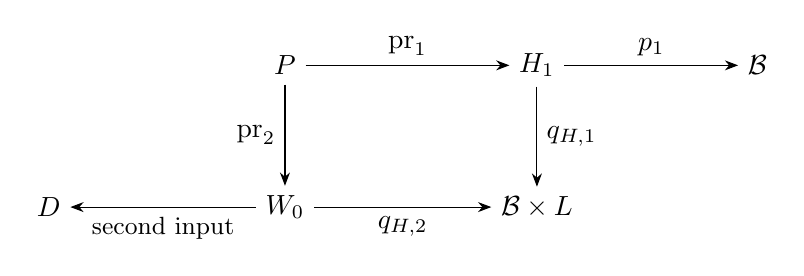
\begin{tikzpicture}[>=Stealth,baseline=(current bounding box.center)]
\node (D) at (0,0) {$D$};
\node (W) at (3,0) {$W_0$};
\node (P) at (3,1.8) {$P$};
\node (H) at (6.2,1.8) {$H_1$};
\node (O) at (6.2,0) {$\cB\times L$};
\node (B) at (9,1.8) {$\cB$};
\draw[->] (P) -- node[above] {$\operatorname{pr}_1$} (H);
\draw[->] (P) -- node[left] {$\operatorname{pr}_2$} (W);
\draw[->] (H) -- node[right] {$q_{H,1}$} (O);
\draw[->] (W) -- node[below] {$q_{H,2}$} (O);
\draw[->] (W) -- node[below] {\small second input} (D);
\draw[->] (H) -- node[above] {$p_1$} (B);
\end{tikzpicture}
\caption{The cartesian square of two modifications with a common output
and leg. The cut is imposed through the left-hand map to $D$; the
coefficient is pulled from the first input at the upper right.
The diagonal section $W_0\to P$ makes the two modifications equal.}
\label{det:figure}
\end{figure}

Let $c:P\to D$ be the projection through $W_0$.  Set
$W=\{f=e\}\subset W_0$ and $P_c=\{f(c)=e\}\subset P$.
The distinguished points are $w=(h,d)$ in $W_s$ and
$a=(h,h,d)$ in $(P_c)_s$.  Products here are over the trait when one is
present.

The output-bundle map $W\to\cB$ is smooth near $w$.  Indeed,
$W_0\to\cB\times L$ is smooth, and
\eqref{det:eq-leg} says that the cut differential, on directions
relative to the output bundle, has the nonzero leg component $\xi$.
The eigenisomorphism therefore implies that the cycles of the pulled-back
Hecke transform vanish at $w$.  In the trait case this is smooth base
change from $\Psi F=0$, followed by the lisse tensor compatibility.  In
the field case $W\to\cB_{S_0}$ is smooth over the function trait, where
$\cB_{S_0}$ is the constant stack.  Pullback of the constant family with
coefficient $F$ therefore has zero vanishing cycles, and tensoring by
the lisse eigenvalue preserves this assertion.  Only the smooth map to the bundle stack enters this argument.

\smallskip\noindent
\emph{2. Isolating one stalk in the proper pushforward.}
Replace $H_1$ by its Schubert bound $\overline H_1$ and let
$\IC_\lambda$ be the simple Satake kernel of this bound. Set
\[
 \overline P_c=\overline H_1\times_{\cB\times L}W,
 \qquad \pi_c:\overline P_c\longrightarrow W.
\]
This map is proper. Let $\mathcal J$ be the pullback to $\overline P_c$
of the Hecke integrand $F\,\widetilde\boxtimes\,\IC_\lambda$ on
$\overline H_1$, with the twisted-product convention of
\eqref{found:hecke}. In the field case extend the integrand constantly
in $z$ before pulling back to the cut; thus $\mathcal J$ is defined on
the whole $z$-family. In the trait case it is defined on the geometric
generic fiber. Proper base change identifies $R\pi_{c,*}\mathcal J$
with the pullback to $W$ of the Hecke transform used in Step~1.

Let $T=\pi_c^{-1}(w)$ and let $C$ be the restriction to $T$ of
$\Phi\mathcal J$ in the field case, or of $\Psi\mathcal J$ in the
trait case. Proper compatibility of cycles and the vanishing in Step~1
give
\begin{equation}\label{det:eq-proper-zero}
                            R\Gamma(T,C)=0.
\end{equation}
On the open stratum $P_c\subset\overline P_c$ the kernel is
$E[m](m/2)$. We will isolate the contribution of $a$ there.

The open part of $T$ is exactly $H_{\mathrm{out}}$ for $H_1$,
since $w$ fixes $H_2=h$ and $c=d$. Thus \eqref{det:eq-leg} at the
fixed second modification identifies $d(f\circ c)$ along this whole
fiber with the pullback of $(A',\xi)$ along $q_{H,1}$.
Before cutting, $P\to\cB$ by the first input bundle is smooth. At a
point of $T$ in its open-orbit neighborhood, failure of smoothness after
cutting would mean that $d(f\circ c)$ comes from the cotangent space of
that first input bundle. Since $P\to H_1$ is smooth, its
cotangent map is injective; thus failure would already give on $H_1$
an equality
\[
                         q_{H,1}^*(A',\xi)=p_1^*A_1
\]
for some $A_1$.  On $\widetilde p_1$-relative tangents this forces
$o_1^*A'$ to vanish.  The nondegenerate zero on $H_{\mathrm{out}}$
shows that $a$ is isolated among such points of $T$.  Consequently $C$
vanishes on a punctured neighborhood of $a$ in $T$: there the cut map
to the first input stack is smooth and the open-orbit Satake kernel is
an invertible constant shift and twist.
This smoothness is over the trait.  In the field case the integrand
therefore pulls back the constant $F$-family on $\cB_{S_0}$, so it has zero
$\Phi$, as required; the trait case uses $\Psi F=0$.

Here is the precise consequence of this isolation.  If a constructible
complex on a proper scheme vanishes on a punctured neighborhood of a
closed point, its contribution at that point is a direct summand of its
global cohomology.  To see this, let $j:T\setminus\{a\}\to T$ and
$i:\{a\}\to T$.  The restriction $j^*C$ is zero near $a$, so
$(Rj_*j^*C)_a=0$.  The localization triangle consequently splits as the
direct sum of $i_*C_a$ and $Rj_*j^*C$; both connecting morphisms vanish
by these disjoint supports.  The same localization argument applies
to algebraic spaces.  Equation
\eqref{det:eq-proper-zero} now gives
\begin{equation}\label{det:eq-vertex-zero}
                                  C_a=0.
\end{equation}

\smallskip\noindent
\emph{3. An exact split quadratic equation at the isolated point.}
We identify the local equation at this isolated point exactly.  The
diagonal $W_0\to P$, given by making the two modifications equal, is a
section of the smooth map $P\to W_0$.  \'Etale locally at $a$, there is a
map $r:P\to D$ lifting the first-input map to $\cB$, whose restriction
to this diagonal is the original chart point, including its
identification with the first input.  Indeed, the smooth morphism
$P\times_{\cB}D\to P$ has that section on the diagonal.  To extend it,
choose relative smooth coordinates, giving an \'etale map from a
neighborhood of its value to $\mathbb A^\delta_P$, where $\delta$ is
the relative dimension of $D\to\cB$ at $d$.  The coordinates of the
prescribed section are functions on the diagonal; lift these functions
to a neighborhood in $P$ and take their graph in $\mathbb A^\delta_P$.
Pullback of the \'etale map along this graph gives an \'etale neighborhood
of $P$ with a lift to $P\times_{\cB}D$.  Retain the branch carrying
the prescribed section along the diagonal.  The resulting projection
to $D$ is $r$, and the fiber product retains the specified stack
isomorphism between $b\circ r$ and the first input.
Thus $c$ records the second input everywhere, whereas $r$ records the
first input in this \'etale neighborhood; the two agree on the diagonal.
The diagonal, being a section of the smooth morphism $P\to W_0$ of
relative dimension $m$, is a regular immersion of codimension $m$.
Choose relative coordinates $v_1,\ldots,v_m$ generating its ideal.
Since $r=c$ on it, there are functions $u_i$ with
\begin{equation}\label{det:eq-exact-uv}
                         f(c)-f(r)=\sum_{i=1}^m u_i v_i.
\end{equation}
In particular, the subsequent change of coordinates will give the exact
cut equation.

On the diagonal fiber with $c=d$ and leg $y$, which is the fixed-input,
fixed-leg fiber of $H$ through $h$, the conormal coefficients
$u_i$ are the negatives of the restriction of $p^*A$ to the
$q_H$-relative tangent, in the frame dual to the $v_i$.  In fact variation
of the first modification with the second fixed has $dc=0$, whereas
$b\circ r$ is its first input, so differentiating
\eqref{det:eq-exact-uv} gives precisely this restriction.  This
calculation is independent of the chart-vertical part of $dr$:
$df_d=b^*A$ annihilates $\ker(db_d)$.
The description holds along that entire diagonal fiber.  The
nondegenerate zero on $H_{\mathrm{in}}$ shows that $u_i(a)=0$ and that the
derivatives of the $u_i$ on that fiber form a basis.  The map
$W_0\to D\times L$ is the smooth base change of $\widetilde p$,
of relative dimension $m$.  On the diagonal,
$r=c$ and the leg provide the other coordinates; the $v_i$ provide its
normal coordinates.  Hence
\begin{equation}\label{det:eq-uv-chart}
 (r,l,u_1,\ldots,u_m,v_1,\ldots,v_m):
 P\longrightarrow D\times L\times\mathbb A^{2m}
\end{equation}
is \'etale near $a$, with the evident relative interpretation over $S_0$.
On this neighborhood of the cut,
$\mathcal J|_{P_c}\simeq r^*K[m](m/2)$. Thus
\eqref{det:eq-vertex-zero} says that the cycles of the pulled-back $K$
vanish at the vertex of
\begin{equation}\label{det:eq-affine-quadric}
                         f+\sum_i u_i v_i=e.
\end{equation}
For $m=0$ this is already the required assertion, after removing the
smooth leg factor.

\smallskip\noindent
\emph{4. Recovering the original hypersurface.}
We have proved vanishing after adjoining the split quadratic variables.
To remove them, we use a proper family whose extra cohomology is
supported precisely on the original cut $\{f=e\}$.
For $m>0$, put $B=D\times L$ and compactify
\eqref{det:eq-affine-quadric} to the proper quadric family
\begin{equation}\label{det:eq-projective-quadric}
 \pi:Q=\left\{\sum_{i=1}^m u_i v_i+(f-e)w^2=0\right\}
               \subset\mathbb P^{2m}_B\longrightarrow B.
\end{equation}
In the field case $B$ also carries the constant extension in $z$.
Every point above $(d,y)$ other than the vertex $[0:\cdots:0:1]$ is
smooth for $\pi$, since some $u_i$ or $v_i$ is nonzero.  The cycles of
$\pi^*K$ there vanish by smooth base change; they vanish at the vertex
by \eqref{det:eq-uv-chart}.  Proper compatibility therefore gives
zero cycles for $R\pi_*\pi^*K$ at $(d,y)$.

The split-quadric calculation in
\cite[proof of Lemma~4.3]{CT} gives the precise extra term we need.
Write $i:Z=\{f=e\}\hookrightarrow B$. Hyperplane powers give a triangle
\begin{equation}\label{det:eq-quadric-triangle}
 \bigoplus_{a=0}^{2m-1}E_B(-a)[-2a]\longrightarrow R\pi_*E_Q
 \longrightarrow i_*E_Z(-m)[-2m]\xrightarrow{+1}.
\end{equation}
Here the first arrow is an isomorphism outside $Z$: a smooth split
quadric of dimension $2m-1$ has the same $E$-cohomology as
$\mathbb P^{2m-1}$. Over $Z$ the family is the constant projective cone
on the split quadric of dimension $2m-2$. Its cohomology has one
additional copy of $E(-m)$ in degree $2m$, beyond the hyperplane
powers. Proper base change identifies the restriction of the cone of
the first arrow with this constant complex on $Z$; localization
therefore identifies the cone as the last term displayed. This explains
why the triangle is a statement about sheaves, not merely fiber
cohomology dimensions.

Tensor \eqref{det:eq-quadric-triangle} with $K$ and use the
projection formula.  In the trait case take this triangle on the
geometric generic fiber.  The cycles of its first term vanish at
$(d,y)$ because $\Psi K=0$; those of its middle term vanish by the
proper calculation above.  Its last term therefore has zero nearby
cycles there, and proper compatibility for $i$ proves the claimed
vanishing on $\{f=0\}$.  In the field case use the triangle on the
whole $z$-family.  Its first term has zero vanishing cycles because
$K$ is pulled from the constant family $D$.  The identical argument
with $\Phi$ proves $(\Phi_f K)_d=0$.  Smooth base change removes the
leg factor in both cases.  The sheaf operations used throughout are
those in Proposition~\ref{found:nearby}.
\end{proof}

\subsection{Nilpotent singular support}

\begin{proof}[Proof of Theorem~\ref{det:field}]
Apply Lemma~\ref{det:cut} on every smooth chart and
every open subchart.  It says that every function whose differential
at a point is outside $\Lambda_D$ is locally acyclic there relative to
$b^*F$.  The cone includes the zero section, so these are precisely the
nonzero directions that must be excluded.  Weak singular support is
the closure of the differentials of functions with nonzero vanishing
cycles; over an infinite field closed-point tests suffice by
constructibility.  Barrett proves this description for the present
$E$-coefficients and proves that weak singular support equals full
singular support \cite[\S\S1.4--1.5, Theorem~(vii)]{Barrett}, extending
Beilinson's torsion-coefficient theorem \cite[\S1.5]{Beilinson}.
The hypersurface calculation therefore gives
$\SS(b^*F)\subset\Lambda_D$.  The same calculation on charts with
additional smooth parameters is available, so the conclusion is
compatible with the smooth-chart definition of singular support on
the stack.
\end{proof}

\subsection{Simultaneous cuts and nonvanishing of specialization}

To prove specialization detection, we must pass from hypersurfaces to
enough simultaneous cuts to make the support finite over the trait.
Successive hypersurface applications would require information about the
singular support of intermediate restrictions.  The following incidence
argument makes all the cuts at once.

\begin{lemma}[Simultaneous cuts]\label{det:simultaneous}
In the trait case, assume $\Psi F=0$.  Let $f_1,\ldots,f_r$ vanish at
$d\in D_s$ and suppose their special-fiber differentials span an
$r$-dimensional subspace $V\subset T_d^*D_s$ with
$V\cap(\Lambda_D)_d=\{0\}$.  Then nearby cycles of
$K|_{\{f_1=\cdots=f_r=0\}_{\bar\eta}}$ vanish at $d$.
The statement for $r=0$ is $\Psi K=0$.
\end{lemma}

\begin{proof}
The case $r=1$ is Lemma~\ref{det:cut}.  For $r>1$
consider the proper incidence projection
\[
 \pi:J=\{(t,[a_1:\cdots:a_r])\in D\times\mathbb P^{r-1}:
                   \textstyle\sum_i a_i f_i(t)=0\}\longrightarrow D.
\]
At $(d,[a])$ the differential of the defining function on a standard
projective chart is $\sum_i a_i df_i$; derivatives in the projective
directions are zero since all $f_i(d)$ vanish.  It is nonzero and lies
outside the pulled-back nilpotent cone.  The map
$D\times\mathbb A^{r-1}\to\cB$ on each such chart is smooth, so
Lemma~\ref{det:cut} proves that the nearby cycles of
$\pi^*K$ vanish on the whole fiber $\mathbb P^{r-1}$ over $d$.
Proper compatibility gives $(\Psi R\pi_*\pi^*K)_d=0$.

Let $i:Z=\{f_1=\cdots=f_r=0\}\hookrightarrow D$.  On the geometric
generic fiber hyperplane powers give the triangle
\[
 \bigoplus_{a=0}^{r-2}E_D(-a)[-2a]\longrightarrow R\pi_*E_J
 \longrightarrow i_*E_Z(-(r-1))[-2(r-1)]\xrightarrow{+1}.
\]
Indeed, over $D\setminus Z$ the incidence is a projective bundle of
relative dimension $r-2$, so the first arrow is an isomorphism there.
Over $Z$ it is the product $Z\times\mathbb P^{r-1}$, and the cone has
only its constant top cohomology sheaf.  Proper base change and
localization identify the cone as written, not merely its stalk
dimensions.  Tensor by $K$.  The first term has zero nearby cycles by
$\Psi K=0$, and the middle term by the preceding proper calculation.
Proper compatibility for $i$ proves the lemma.
\end{proof}

\begin{proof}[Proof of Theorem~\ref{det:specialization}]
Suppose that the closure of the nonzero-stalk locus meets $D_s$.
Shrink to an affine chart smooth of constant relative dimension $N$ over
$S_0$.  The
closure of that locus in $D_{\bar\eta}$ has finitely many irreducible
components $Z_{\bar\eta,\alpha}$.  Constructibility gives, on each
component, a dense open subset where the stalk of $K$ is nonzero.
After a finite extension of the trait, descend the components and the
proper closed complements of these opens.  We only descend these finite
algebraic data, and continue to use $K$ over $\bar\eta$.
Let $Z_\alpha\subset D$ and $E_\alpha\subset Z_\alpha$ be their
horizontal closures.  Components not meeting $D_s$ may be removed.

Write $j$ for the largest dimension of a generic component whose
closure meets $D_s$, and choose an irreducible component $Z_0$ of the
reduced special fiber of such a closure.  A horizontal integral
finite-type scheme over this excellent trait, with generic dimension
$j$, has every nonempty special-fiber component of dimension $j$;
its local dimension at a special-fiber closed point is $j+1$.
For these two assertions see, respectively,
\cite[Tags 0B2J and 02JU]{Stacks}.  The same dimension calculation
shows that the special fibers of the horizontal exceptional closures
$E_\alpha$ have dimension at most $j-1$ whenever the corresponding
generic component has dimension at most $j$.

Choose a general closed point $d$ of $Z_0$.  We may arrange that $Z_0$
is smooth at $d$, that $d$ is in none of the exceptional closures,
and that every reduced special-fiber component of the support closure
through $d$ equals $Z_0$ near $d$.  Distinct horizontal components may
have this same special component; this causes no difficulty.  By
Proposition~\ref{geom:dimension},
\[
                  \dim\Lambda_D\leq N.
\]
After shrinking a dense open in $Z_0$, the fiber dimension theorem
therefore gives
\begin{equation}\label{det:eq-cone-fiber}
                    \dim(\Lambda_D)_d\leq N-j.
\end{equation}

Choose a $j$-plane $V\subset T_d^*D_s$ which avoids
$(\Lambda_D)_d\setminus\{0\}$ and whose restriction to $T_dZ_0$
is an isomorphism onto $T_d^*Z_0$.  Both are nonempty open conditions
on the Grassmannian.  When $j>0$, for the first condition projectivize the cone in
\eqref{det:eq-cone-fiber}: it has dimension at most $N-j-1$,
and a general $\mathbb P^{j-1}$ in $\mathbb P^{N-1}$ is disjoint
from it by the elementary incidence dimension count.  The second is
the usual complement-to-a-fixed-subspace condition.  The base field
is infinite, so the two opens meet.  If $j=0$, take $V=0$ and use no
cutting functions.  Lift a basis of $V$ to
differentials of regular functions $f_1,\ldots,f_j$ vanishing at $d$.
Their restrictions are parameters on the smooth scheme $Z_0$.
Put $Y=\{f_1=\cdots=f_j=0\}\subset D$.
Lemma~\ref{det:simultaneous} says
\begin{equation}\label{det:eq-final-zero}
                         (\Psi(K|_{Y_{\bar\eta}}))_d=0.
\end{equation}

We finish by showing directly that this stalk is nonzero.  Near $d$,
the special fiber of the closed support closure intersected with $Y$
is zero-dimensional.  On any of its selected horizontal components
$Z_\alpha$ of generic dimension $j$ through $d$, the local ring has
dimension $j+1$, so its quotient by the $j$ functions has dimension
at least one \cite[Tag 0B52]{Stacks}.  Its further quotient by the uniformizer is
zero-dimensional.  Thus this intersection has a generization of $d$
in the generic fiber.  Such a generization lies outside $E_\alpha$,
since $d$ was chosen outside its closure, and $K$ has a nonzero
geometric stalk there.

For completeness, the passage from this generization to nearby cycles
is local and finite.  Let $Z\subset Y$ be the reduced intersection
$Y\cap\bigcup_\alpha Z_\alpha$.  Its generic fiber contains the
nonzero-stalk locus of $K|_{Y_{\bar\eta}}$, the preceding generization
lies in $Z$, and $d$ is isolated in $Z_s$.
The morphism $Z\to S_0$ is quasi-finite at $d$.
Take an affine neighborhood in $Y$ and use the henselian decomposition
of its closed support: the local ring of $Z$ at $d$ is a finite local
$R$-algebra and defines an open-and-closed piece $T\subset Z$
\cite[Tag 04GH(3) and its proof]{Stacks}.  Its unique special-fiber
point is $d$.  Remove the closed complement $Z\setminus T$ from the
ambient neighborhood.  On the resulting neighborhood, which has the
same nearby-cycle stalk at $d$, the support closure is the finite
$S_0$-scheme $T$.

The generic restriction of $K$ is the extension by zero from this
finite closed support.  Proper base change now identifies its
nearby-cycle stalk at $d$ with
\[
               \bigoplus_{z\in T_{\bar\eta}}
                             (K|_{Y_{\bar\eta}})_z.
\]
This is a finite direct sum of complexes of $E$-vector spaces, at
least one of which is nonzero.  Hence the sum is nonzero, contradicting
\eqref{det:eq-final-zero}.  The argument includes $j=0$, when
there are no cutting functions and the original support already has
the required finite local piece.  This proves the theorem.
\end{proof}

\section{Perverse cohomology of a dense eigencomplex}
\label{perv:section}

We now work over $\mathbb C$.  Our objective is to extract a perverse
object from an eigencomplex without losing its moving-leg eigenmaps or
fusion constraints.  Density makes the spectral parameter a free closed
orbit.  A frame along this orbit gives exactness of fixed-point Hecke
operators on a subcategory containing the eigencomplex and its
truncations; local constancy in the legs then supplies the moving
statement.  This is the argument of \cite[\S6]{CT}, with all the marked
points retained in the level structure.

Let $X/\mathbb C$ be a smooth projective connected curve of genus $g$,
let $D=x_1+\cdots+x_s$ be a nonempty reduced divisor, and put
$U=X\setminus |D|$.  Let $\cB$ be either $\cA$ or $\cA^+$ from
Section~\ref{found:level-stacks}, and let $\Lambda\subset T^*\cB$
be its generically nilpotent cone from Section~\ref{geom:section}.
All Hecke functors use the relative Satake normalization.

\begin{proposition}\label{perv:eigen}
Suppose $F\in\Dlc(\cB,E)$ is a coherent Hecke eigencomplex for a
continuous parameter
$\sigma:\pi_1^{\et}(U)\to\Gd(L)$ with Zariski-dense image, where
$L/\mathbb Q_\ell$ is finite.  Then every ${}^pH^j(F)$ has a natural
coherent eigenstructure for $\sigma$, with singular support in $\Lambda$.
The eigenmaps are natural in representations and compatible with the
unit, convolution, permutations, and fusion on every collision diagonal.
If $F\ne0$, some ${}^pH^j(F)$ is nonzero.  No global cohomological bound
on $F$ and no condition on the boundary monodromy are required.
\end{proposition}

\subsection{The Betti spectral action with all levels present}

We state the Betti input before using it.  At each $x_i$, in a formal
coordinate $t_i$, ordinary and enhanced flags correspond respectively to
\[
 \mathrm{Iw}_i=\{h\in G(\mathbb C[[t_i]]):h(0)\in B\},\qquad
 \mathrm{Iw}_i^0=\{h\in G(\mathbb C[[t_i]]):h(0)\in N_B\}.
\]
The first congruence subgroup is normal in each of these groups, and
both groups lie in the positive-loop maximal parahoric, hence in its
normalizer.  Thus the finite set of levels satisfies the
hypotheses of Nadler--Yun's level-structure results
\cite[\S6.2]{NY}.  Their level cotangent nilpotent cone is defined by
generic nilpotence and is exactly $\Lambda$, with the residue conditions
established in Section~\ref{geom:section}.

Write $\mathscr D_\Lambda(\cB)$ for the Betti category with singular
support in this cone.  The results of
\cite[Theorem~6.2.2, Proposition~6.3.2, \S6.3.6, and Theorem~6.3.7]{NY}
give the following two inputs.
First, for a finite set $I$ and representations
$\boldsymbol V=(V_i)_{i\in I}$, the moving transform satisfies
\begin{equation}\label{perv:leg-support}
 \SS\bigl(\Hecke_{I,\boldsymbol V}(K)\bigr)
       \subset \Lambda\times 0_{U^I},
       \qquad K\in\mathscr D_\Lambda(\cB).
\end{equation}
This holds on the full product, including collisions.  On smooth charts,
the isotropy proved in Section~\ref{geom:section} and the
product-stratification argument in the proof of
\cite[Proposition~6.3.2 and \S6.3.6]{NY} make
this a local product statement.  On each finite-type smooth chart,
choose a microlocal stratification whose conormals contain the
pulled-back cone.  The output is weakly constructible for its product with a
sufficiently small contractible analytic leg patch, and hence is the
pullback of a fixed-leg slice.
The transport is compatible with the Hecke tensor operations.

Second, choose $u\in U^{\mathrm{an}}$ and free generators
$\gamma_1,\ldots,\gamma_a$ of its topological fundamental group, where
$a=2g+s-1$.  Since $U^{\mathrm{an}}$ has the homotopy type of a bouquet
of these circles, its Betti stack of $\Gd$-local systems is
\[
 \mathscr L=[Y/\Gd],\qquad Y=\Gd^{a},
\]
with simultaneous conjugation.  The symmetric monoidal category
$\Perf(\mathscr L)$ acts on $\mathscr D_\Lambda(\cB)$.  For
$V\in\Rep_E(\Gd)$, the equivariant bundle
$\mathscr E_V=Y\times V$ acts by $\Hecke_{V,u}$; its tautological
automorphisms along the $\gamma_i$ act by Hecke transport
\cite[Proposition~6.3.3 and \S6.3.6]{NY}.
These statements use the Satake labeling fixed in
Section~\ref{found:section}.

The Betti categories in \cite[\S5.1 and \S6.2]{NY} do not impose global
boundedness or support in a finite-type substack.  The Hecke transforms
above preserve local bounded constructibility: on any finite-type output
chart a Satake kernel has a finite-dimensional bound, whose proper
correspondence meets only a quasi-compact part of the input stack.
Consequently the local product statement also applies to the lcc objects
and to the finite diagrams used below, locally on finite-type charts.

\begin{lemma}[The scalar spectral action]\label{perv:scalar}
Let $K\in\mathscr D_\Lambda(\cB)$ have a coherent Betti eigenstructure
with parameter represented by $y\in Y(E)$.  Every
$f\in E[Y]^{\Gd}$ acts, as a degree-zero endomorphism of the spectral
unit and hence of $K$, by $f(y)\operatorname{id}_K$.
\end{lemma}

\begin{proof}
We use the identification with excursion operators in
\cite[\S7.1 and Proposition~7.2.3]{NY}; the scalar calculation is
\cite[Lemma~6.2]{CT}.  Here is the calculation for the free group of
rank $2g+s-1$.  Matrix coefficients span $E[Y]$.  Exactness of
invariants for the reductive group $\Gd$ implies that every invariant
is a finite sum of functions
\begin{equation}\label{perv:excursion}
 (g_1,\ldots,g_a)\longmapsto
 \operatorname{Tr}_{W}\left(A\circ\bigotimes_{i=1}^{a}V_i(g_i)\right),
 \qquad W=\bigotimes_{i=1}^{a}V_i,\quad
 A\in\operatorname{End}_{\Gd}(W).
\end{equation}
Indeed products of matrix coefficients are images of
$\operatorname{End}_E(W)$ under this trace map.  A finite sum of these
finite-dimensional equivariant images contains a prescribed invariant;
exactness of invariants lifts it to invariant endomorphisms in the
corresponding finite sum of source spaces.

The excursion for \eqref{perv:excursion} inserts the coevaluation tensor
in $W\otimes W^*$, transports each $V_i$ around $\gamma_i$, applies
$A$, and evaluates.  The dual factor can remain at $u$ as an identity
leg.  Naturality, the tensor constraints, and the unit constraint of the
eigenstructure identify this operation with the same tensor calculation
on the parameter.  Its value is \eqref{perv:excursion} at $y$.
This proves the assertion for every invariant function.  In particular
the scalar follows from the coherent eigenmaps, not merely from
fixed-point eigenisomorphisms.
\end{proof}

\subsection{Equivariant frames and exactness}

The next algebraic lemma trivializes each $\mathscr E_V$ after inverting
an invariant function nonzero at a given dense parameter.
Its frames will be used only to prove
exactness.  They need not respect tensor products, since the eigenmaps
will be obtained by truncating the original coherent maps.

\begin{lemma}\label{perv:frame}
If the entries of $y\in Y(E)$ generate a Zariski-dense subgroup of
$\Gd=\mathrm{PGL}_{n,E}$, then for every nonzero representation $V$,
of dimension $b$, there are an invariant $f_V\in E[Y]^{\Gd}$ with
$f_V(y)\ne0$ and equivariant maps
\[
 \alpha_V:\mathcal O_Y^{\oplus b}\longrightarrow\mathscr E_V,
 \qquad
 \beta_V:\mathscr E_V\longrightarrow\mathcal O_Y^{\oplus b}
\]
such that
\begin{equation}\label{perv:adjugates}
 \beta_V\alpha_V=f_V\operatorname{id},\qquad
 \alpha_V\beta_V=f_V\operatorname{id}.
\end{equation}
\end{lemma}

\begin{proof}
This is the closed-orbit frame argument of \cite[Lemma~6.3]{CT}.
The stabilizer of $y$ is the centralizer of a dense subgroup, hence
$Z(\Gd)=1$.  Its orbit $O$ is closed: a one-parameter subgroup giving
a limit of the conjugated tuple forces every entry into its associated
parabolic.  Density forces that parabolic to be all of $\Gd$, so the
one-parameter subgroup is central.  The affine Hilbert--Mumford
closed-orbit criterion proves the claim.  Thus $O\simeq\Gd$.

A basis $v_1,\ldots,v_b$ at $y$ defines equivariant sections on $O$ by
$s_j(hy)=hv_j$.  Restriction
$E[Y]\otimes V\twoheadrightarrow E[O]\otimes V$ is surjective because
$O$ is closed and $Y$ is affine.  Reductivity in characteristic zero
makes invariants exact, so these sections extend equivariantly to $Y$.
Use the extensions as the columns of $\alpha_V$.
Every character of the semisimple group $\Gd$ is trivial, so
$\det V$ is trivial.  After choosing a volume form,
$f_V=\det\alpha_V$ is invariant and nonzero at $y$.
The adjugate defines a regular equivariant map $\beta_V$ on all of $Y$:
on the dense open set $f_V\ne0$ it equals $f_V\alpha_V^{-1}$, and
this identity verifies equivariance everywhere.  The two adjugate
identities give \eqref{perv:adjugates}.
\end{proof}

Let $\mathscr D^{\mathrm{lcc}}_\Lambda(\cB)$ be the lcc part of the
Betti nilpotent category.  It is stable under perverse truncation.
Locally this is the microlocal d\'evissage assertion that the singular
support of a bounded complex is the union of the singular supports of
its perverse cohomologies; it follows equivalently from the exact
perverse vanishing-cycle tests.  Smooth charts give the statement
without a uniform bound on the stack.

Fix a dense tuple $y$ as in Lemma~\ref{perv:frame}.  For each
isomorphism class of nonzero representations choose $f_V$ supplied by
that lemma for this tuple, and let $S$ be the multiplicative set they
generate.  Define
\[
 \mathscr D_S=\{K\in\mathscr D^{\mathrm{lcc}}_\Lambda(\cB):
             f_K:K\to K\text{ is invertible for every }f\in S\}.
\]
Here $f_K$ denotes the central endomorphism given by the spectral action.

\begin{lemma}\label{perv:exact}
The subcategory $\mathscr D_S$ is preserved by perverse truncations and
by all fixed-point Hecke functors.  Every fixed-point Hecke functor is
perverse $t$-exact on this subcategory.
\end{lemma}

\begin{proof}
For a degree-zero natural endomorphism $f$ of the identity, naturality
for ${}^p\tau_{\le r}K\to K$ and the universal property of truncation give
\[
 f_{{}^p\tau_{\le r}K}={}^p\tau_{\le r}(f_K).
\]
Indeed both sides are the unique endomorphism of the truncation whose
composite to $K$ equals $f_K$ after the truncation map.  The other
truncation has the analogous property.  Invertibility therefore passes
to both truncations, proving that $\mathscr D_S$ inherits the perverse
$t$-structure.  No exactness of an arbitrary spectral operator has been
assumed.

Applying the spectral action to \eqref{perv:adjugates} gives maps
\[
 K^{\oplus b}\xrightarrow{\alpha_{V,K}}\Hecke_{V,u}(K)
                \xrightarrow{\beta_{V,K}}K^{\oplus b}.
\]
Symmetric monoidality identifies $f_{\Hecke_{V,u}(K)}$ with
$\Hecke_{V,u}(f_K)$, so the Hecke functor preserves $\mathscr D_S$.
On this subcategory the adjugate identities make $f_V^{-1}\beta_{V,K}$
an inverse to $\alpha_{V,K}$.  Hence
\begin{equation}\label{perv:fixed-exact}
 \Hecke_{V,u}|_{\mathscr D_S}
          \simeq\operatorname{id}_{\mathscr D_S}^{\oplus\dim V},
\end{equation}
which proves exactness.  Hecke transport along a path from $u$ proves
the assertion at any allowed point.  The zero representation acts by
zero.  Compositions, including convolution at a shared point, are
therefore exact and preserve $\mathscr D_S$ as well.
\end{proof}

\subsection{Moving legs, collisions, and adic eigenmaps}

\begin{proof}[Proof of Proposition~\ref{perv:eigen}]
Let $K$ be the Betti realization of $F$, using
Section~\ref{found:betti}.  Theorem~\ref{det:field} and singular-support
comparison put $K$ in $\mathscr D^{\mathrm{lcc}}_\Lambda(\cB)$.
Its topological monodromy remains Zariski dense.  The topological
fundamental group has dense image in the profinite fundamental group;
a polynomial equation on the image, after adjoining its coefficients
to a finite extension of $L$, is closed for the adic topology.  An
equation on topological monodromy therefore holds on the entire adic
image.  The tuple $y$ associated with $K$ satisfies
Lemma~\ref{perv:frame}; use this tuple to choose $S$ and $\mathscr D_S$.
By Lemma~\ref{perv:scalar},
$f_{V,K}=f_V(y)\operatorname{id}_K$, so $K\in\mathscr D_S$.
Lemma~\ref{perv:exact} puts all of its perverse truncations and
cohomologies in this subcategory.

We first prove the bounds needed to truncate moving transforms.
For $A\in\mathscr D_S$ and $m=|I|$, the functor
\[
                 A\longmapsto\Hecke_{I,\boldsymbol V}(A)[m]
\]
is perverse $t$-exact.  On a contractible leg patch,
\eqref{perv:leg-support} identifies its unshifted value with a constant
family of fixed-point transforms.  The fiber is a composition of
fixed-point Hecke functors, using convolution where the legs coincide,
and hence has the bounds of $A$ by Lemma~\ref{perv:exact}.
The constant sheaf shifted by $m$ on the smooth parameter space is
perverse.  The product description therefore proves the asserted bounds
on smooth charts.  Applying this exact functor to a truncation triangle
and using its universal property yields natural isomorphisms
\begin{equation}\label{perv:moving-truncation}
 {}^pH^j\bigl(\Hecke_{I,\boldsymbol V}(A)[m]\bigr)
       \simeq\Hecke_{I,\boldsymbol V}({}^pH^jA)[m].
\end{equation}

The same bounds hold for successive operations with all previous leg
variables retained.  Locally in those variables the input is a constant
family whose fixed-leg fibers belong to $\mathscr D_S$.  Applying the
next Hecke operator uses \eqref{perv:fixed-exact} on these fibers and
\eqref{perv:leg-support} for its parameter dependence.  Thus the
truncation comparison holds throughout each composition diagram.
The shift is the dimension of the total retained parameter space,
counted once; successive operations at a shared leg add no parameter.

For clarity, let $\pi:I\twoheadrightarrow J$ be a surjection, let
$\Delta_\pi:U^J\to U^I$ be its collision diagonal, and put
$W_j=\bigotimes_{i\in\pi^{-1}(j)}V_i$.  The fusion convention gives
\[
 (1\times\Delta_\pi)^*\Hecke_{I,\boldsymbol V}(A)
                  \simeq\Hecke_{J,\boldsymbol W}(A).
\]
On the local product families just considered,
\begin{equation}\label{perv:collision-exact}
                  (1\times\Delta_\pi)^*[\,|J|-|I|\,]
\end{equation}
is perverse exact: it replaces a perverse constant factor on a smooth
$|I|$-dimensional base by the perverse constant factor on the
$|J|$-dimensional base.  This proves compatibility of
\eqref{perv:moving-truncation} with collision restriction, including
iterated collisions.  Local constancy only away from diagonals would
not suffice for this step.

These bounds construct the required comparisons in the adic category
itself.  Start with the adic truncation triangles of $F$ and apply the
adic Hecke functors.  Betti realization preserves perversity and is
conservative on the finite-type charts, so the bounds just proved show
that their images are truncation triangles.  Their universal property
therefore supplies \eqref{perv:moving-truncation} adically for $F$.
The same argument applies to the retained-leg compositions and the
shifted diagonal restriction \eqref{perv:collision-exact}.
In particular no algebraization of maps constructed only in the Betti
category is needed.

Write $\mathcal V_{I,\sigma}=\boxtimes_{i\in I}(V_i)_\sigma$.
Shift the original adic eigenmap by $m$, apply ${}^pH^j$, and use
\eqref{perv:moving-truncation}.  Exterior product with the lisse factor
$\mathcal V_{I,\sigma}[m]$ is perverse exact.  We obtain
\[
 \Hecke_{I,\boldsymbol V}({}^pH^jF)[m]
       \simeq({}^pH^jF\boxtimes\mathcal V_{I,\sigma})[m].
\]
Removing the common shift gives precisely the required eigenmap
\begin{equation}\label{perv:induced-eigen}
 \Hecke_{I,\boldsymbol V}({}^pH^jF)
                  \simeq{}^pH^jF\boxtimes\mathcal V_{I,\sigma},
\end{equation}
with no moving-leg shift.

Finally apply the functorial truncation comparisons to the diagrams of
the original coherent eigenstructure.  Naturality in representations,
the unit, and permutations commute with truncation.  The retained-leg
comparison proves compatibility with convolution, and
\eqref{perv:collision-exact} proves compatibility with fusion.
Every vertex over $U^I$, after the single shift $[|I|]$, lies in the
perverse heart: locally it is a fixed-point exact transform of
${}^pH^jF$ times a lisse parameter factor.  After collision to $U^J$,
the adjustment $[|J|-|I|]$ places all vertices in the new heart.
For objects $P,Q$ of such a heart,
$\pi_r\operatorname{Map}(P,Q)=\operatorname{Hom}(P,Q[-r])=0$ for
$r>0$.  Thus their mapping spaces are discrete, and the commutative
diagrams give all the coherent constraints.  The auxiliary choices of
frames played no role in constructing \eqref{perv:induced-eigen}.

Theorem~\ref{det:field} applied to these eigenmaps gives singular
support in $\Lambda$; one may also use perverse microlocal d\'evissage.
All bounds and comparisons were local on finite-type smooth charts.
If $F$ is nonzero, its bounded restriction to some such chart has
nonzero perverse cohomology.  Smooth perverse pullback identifies this
with a restriction of some ${}^pH^jF$, proving nonvanishing.
\end{proof}

\section{Removing all flag enhancements}\label{desc:section}

Work over $\mathbb C$, with the marked curve $(X;x_1,\ldots,x_s)$
and $U=X\setminus\{x_1,\ldots,x_s\}$.  For a parameter $\sigma$
on $U$, write $V_\sigma$ for its associated tensor local system.
We will pass from a nonzero
coherent eigencomplex on $\cA^+$ to a nonzero perverse eigenobject on
$\cA$.  The map
\[
                         q:\cA^+\longrightarrow\cA
\]
is a torsor under $H=T^s$.  Compactly supported direct image along
$q$ can kill a local system with nontrivial torus characters.  The
point of the argument is that unipotent boundary monodromy of the
eigenvalue forces unipotent monodromy along every factor of $H$.

We adapt the one-point descent argument of \cite[Section~7]{CT}.
Its local input is Gaitsgory's central-sheaf construction
\cite{GaitsgoryCentral} in the universal monodromic form of
Dhillon--Taylor \cite{DT}.  The extension needed here keeps the levels
at the other marked points \emph{transported} in every moving and
convolution correspondence.  We spell out the resulting natural
comparisons: the trace identity needs monodromy on one convolution
factor at a time.  The universal kernels occur only in Betti sheaves;
$q_!$ and the final perverse cohomology are operations on the original
geometric adic complexes.

\subsection{Monodromy on the full enhancement torus}

A complex on an $H$-torsor is \emph{monodromic along the torsor} if,
locally on its base, it is constructible for a product stratification
$\{S_\alpha\times H\}$ and, on a contractible patch of $H$, is pulled
back from a slice.  This includes the extension data between strata.
It allows arbitrary monodromy in $\pi_1(H)=X_*(T)^s$ and requires no
equivariant structure.  The condition is preserved by base change on
the base.

\begin{lemma}\label{desc:monodromic}
If $Q\in\Dlc(\cA^+,E)$ has nilpotent singular support, its Betti
realization is monodromic along the whole $T^s$-torsor $q$, and along
each enhancement separately.
\end{lemma}

\begin{proof}
By the cone description following Definition~\ref{geom:cone}, the
nilpotent cone on $\cA^+$ is the
smooth cotangent pullback of the ordinary-level cone: a nilpotent
Borel-valued residue has zero toral component at every marked point.
On a smooth torsor chart $S\times H$ the singular support is therefore
contained in $\Lambda_S\times0_H$.  The cone $\Lambda_S$ is isotropic
by Proposition~\ref{geom:dimension}.  Choose a microlocal
stratification of $S$ whose conormals contain it.  The product
stratification criterion used in \cite[proof of Proposition~6.3.2]{NY} and
\cite[Lemma~7.1]{CT} makes $Q$ constructible for
$\{S_\alpha\times H\}$.  Restriction to a slice over a contractible
patch of $H$ is an equivalence for this constructible category; hence
it identifies the entire complex with the pullback from that slice.
Continuation gives the assertion on overlaps.  These descriptions
persist under base change and, in particular, under passage to the
base of a single enhancement torus.
\end{proof}

\subsection{The single-disc inputs}

Fix one marked point $x_i$.  In this subsection $T$ denotes its
individual enhancement torus; put
\[
 d=\dim T,\qquad \Gamma=X_*(T),\qquad
 R_T=E[\Gamma]=\mathcal O(\widehat T).
\]
Here $\widehat T\subset\Gd$ is the dual maximal torus.
We fix positive cocharacter loops and orientations of the compact
real torus in $T(\mathbb C)$.  Let $\mathscr L_T$ be the local system
with fiber $R_T$ and regular monodromy.  It has infinite-dimensional
stalks and is used in the category of weakly constructible Betti
sheaves.  For ordinary-direct-image convolution its unit is
\begin{equation}\label{desc:unit}
                         \mathbf1_T=\mathscr L_T[d].
\end{equation}
Our enhancement-difference convention writes the varying input as
$e a^{-1}$ for fixed output $e$ and difference $a\in T$.

We use the following precise features of this unit, proved in
\cite[Lemma~7.2]{CT}.  Convolution with $\mathbf1_T$ is naturally the
identity on relatively monodromic complexes, commutes with base
change, and respects successive convolutions.  Multiplication by
$R_T$ on the unit acts as enhancement monodromy.  In fact, if $W$ is
a fiber and $M_1,\ldots,M_d$ its commuting monodromies, the unit
integral before shifting is the Koszul complex
\[
 K^\bullet(z_1M_1^{-1}-1,\ldots,z_dM_d^{-1}-1;
                                      R_T\otimes_E W).
\]
Its cohomology is $W$ in degree $d$, with residual $z_j$ acting by
$M_j$.  This also applies to complexes relatively over a stratified
base.  Compatibility with two integrations follows on the real
universal covers of the compact tori: replace two lifted differences
by the first and their sum, and integrate in that order.  The change
preserves product orientation and continuation follows the same
summed path.  This specifies the unit maps, rather than only their
isomorphism classes.

Let $\mathrm{Iw}$ and $\mathrm{Iw}^0$ be the inverse images of $B$ and
$N_B$ in $L^+G$.  The local central-sheaf input is the monoidal functor
\[
 Z:\Rep(\Gd)\longrightarrow\mathcal H^{\mathrm{mon}},\qquad V\longmapsto Z(V),
\]
where $\mathcal H^{\mathrm{mon}}$ is the universal monodromic Betti
Hecke category on $LG/\mathrm{Iw}^0$, with the pro-unipotent
equivariance convention of \cite{DT}.  It comes with nearby-cycle
monodromies $m_V$, natural in $V$.  We use the kernel specialization
and monoidal comparison of \cite[Proposition~6.3.1 and
Lemma~6.3.2]{DT}, as recorded in \cite[Sections~7.2 and~7.4]{CT}:
the moving Satake kernel tensored with $\mathbf1_T$ specializes to
$Z(V)$, and the specialized twisted product and its convolution map
are the specified monoidal maps of $Z$.

The corresponding local trace formula is
\begin{equation}\label{desc:local-trace}
 \left(\mathbf1_T\xrightarrow{\mathrm{coev}}Z(V)\star Z(V^*)
 \xrightarrow{m_V\star\mathrm{id}}Z(V)\star Z(V^*)
 \xrightarrow{\mathrm{ev}}\mathbf1_T\right)
                 =\chi_V\in\operatorname{End}(\mathbf1_T)=R_T,
\end{equation}
where $\chi_V$ is the character on $\widehat T$ and evaluation in this
order is induced from the symmetric representation category.
For completeness, \cite[Propositions~5.3.1 and~9.3.1(a)--(c)]{DT}
compute this trace after the Wakimoto associated-graded functor.
On the weight summand $\nu\in X^*(\widehat T)=\Gamma$, monodromy is
multiplication by $e^\nu$.  The trace is thus
$\sum_\nu\dim(V_\nu)e^\nu=\chi_V$.  On endomorphisms of the unit the
associated-graded functor retains multiplication on its regular
$R_T$-module, and is faithful there, proving
\eqref{desc:local-trace}.  Reversing conventions inverts both the
torus and boundary loops and does not change the unipotence conclusion.

One further input explains why ordinary pushforward can be
specialized in these correspondences.  We state it because its
hypothesis must be checked again when the other levels are present.

\begin{lemma}[Exchange through an enhancement torus]\label{desc:exchange}
Let $P\xrightarrow{\pi}C\xrightarrow{b}Y$ be a factorization over an
analytic disc $\Delta$, with $\pi$ a torus torsor on the entire family
and $b$ proper.  On finite-dimensional paracompact charts suppose that
$F$ over $\Delta^*$ is weakly constructible and relatively monodromic
along $\pi$.  Then the natural exchange
\begin{equation}\label{desc:push-exchange}
            \Psi(b\pi)_*F\longrightarrow(b_0\pi_0)_*\Psi F
\end{equation}
is an isomorphism.  Base change and projection formula for these
pushforwards also hold, and the comparisons respect composition.
Here $\Psi$ denotes geometric Betti nearby cycles, without taking
monodromy invariants.
\end{lemma}

\begin{proof}
This is \cite[Lemma~7.3]{CT}.  Quotient the enhancement torus by its
positive real radial subgroup $A\simeq\mathbb R^d$, to factor
$P\xrightarrow{\rho}\overline P\xrightarrow{\bar\pi}C$ over the
\emph{whole} disc.  The second map is a compact-torus bundle and
therefore proper.  Relative monodromicity gives
$F=\rho^*\overline F$: restriction across a contractible radial
factor is an equivalence, so the local descriptions glue.  In
trivializations extending across zero,
\[
 R\rho_*\rho^*\overline F=\overline F,
            \qquad \Psi F=\rho_0^*\Psi\overline F.
\]
These identities persist after base change and tensoring with a
factor from the target.  Proper base change for $b\bar\pi$ proves
all assertions.  The maps are the natural exchanges for restriction
and direct image from the universal cover of $\Delta^*$, so they
respect composition.  The same proof applies to products of tori.
\end{proof}

\subsection{A central action with all the other levels retained}

Choose a disc $\Delta$ about $x_i$, disjoint from the other marks,
and a lift to the universal cover of $\Delta^*$.  For the eigenvalue
$V_\sigma$, write $V_{\partial i}$ for the resulting boundary fiber
and $M_{V,i}$ for positive-loop monodromy.  Let $\mu_i$ denote the
$R_T$-action given by continuation along the $i$th enhancement.

\begin{lemma}[Trace at one of several marked points]\label{desc:trace}
Let $Q$ be a locally bounded algebraically constructible Betti
complex on $\cA^+$, monodromic along $T^s$,
with coherent Hecke eigenisomorphisms for $\sigma$ on $U$.  The local
central kernels at $x_i$ act on $Q$, and there are natural
isomorphisms
\begin{equation}\label{desc:central-eigen}
          Z(V)\star_{x_i}Q\simeq Q\otimes_E V_{\partial i}
\end{equation}
compatible with the unit, representation morphisms, and convolution.
On each individual convolution factor they carry $m_V$ to $M_{V,i}$.
In particular, for every $i$ and every $V\in\Rep(\Gd)$,
\begin{equation}\label{desc:character-trace}
              \chi_V(\mu_i)=\operatorname{Tr}(M_{V,i})\,\mathrm{id}_Q.
\end{equation}
\end{lemma}

\begin{proof}
We give the several-level version of \cite[Lemma~7.4]{CT}, including
the comparisons needed to apply \eqref{desc:local-trace}.

\emph{Moving correspondence and its single-step comparison.}
Let $\mathfrak H_{i,\Delta}$ parametrize a leg $z\in\Delta$, two
bundles $P_0,P_1$ with enhancements $\eta_{0j},\eta_{1j}$ at every
$x_j$, and a modification $P_0\simeq P_1$ off $z$.  At $x_i$ the two
enhancements are independent.  At each $x_j$ with $j\ne i$ require
$\eta_{1j}$ to be the transport of $\eta_{0j}$.  Write $p$ for input
and $o$ for output-and-leg.  We bound the underlying modifications
by closed spherical Schubert bounds, retaining the full independent
flags at $x_i$.  Choose these bounds to contain the Satake supports;
their closed central fibers then contain the specialized supports.

Forgetting the levels at $j\ne i$ makes this the pullback of the
one-point moving correspondence by the stack of those levels on
its input.  Transport gives the same description using its output.
This cartesian assertion also holds for successive modifications:
there is one choice of each other enhancement, and the intermediate
and final choices are determined.  It does \emph{not} assert that
$Q$ is pulled back from the one-point stack.

In an input frame compatible with $\eta_{0i}$ the local family is
the one used to define $Z$: its punctured fiber is
$\Gr_G\times G/N_B$ and its central fiber is $LG/\mathrm{Iw}^0$.
The kernel $K_V$ on the punctured fiber is the relative Satake
kernel on $\Gr_G$, tensored with $\mathbf1_T$ on
$T=B/N_B\subset G/N_B$, extended by zero.  Thus it requires equality
of the two ordinary flags at $x_i$ and records their enhancement
difference.  Its specialization is $Z(V)$.  With the relative
normalization of Section~\ref{found:section}, the moving-leg
perverse shift is absent on both sides of this statement.

The kernels and their maps descend from these frames.  On a bound
one can take finite jets on a sufficiently thick neighborhood of
the sum of the graphs of $x_i$ and $z$, so the same smooth frame
space works at collision.  The equivariance of Satake and the
$N_B$-invariance of the flag factor give descent off zero; at zero
it is the $\mathrm{Iw}^0$-equivariance of $Z(V)$.  The finite jet
quotients of this last group are unipotent, hence Betti contractible,
so descent retains the maps and their cocycles.  The extra levels
are outside this neighborhood and enter only in the bundle factor.

For an input family $D$ over $\Delta^*$, write
\[
 A_V(D)=o_*(D\,\widetilde\boxtimes K_V),
                 \qquad B_V(R)=Z(V)\star_{x_i}R,
\]
where the twisted product includes the fixed relative normalization.
For $Q$ viewed as a constant family, the unit calculation gives
\begin{equation}\label{desc:punctured-action}
 A_V(Q)\simeq\Hecke_V(Q)|_{\Delta^*}
                    \simeq Q\boxtimes V_\sigma|_{\Delta^*}.
\end{equation}
Indeed the only integration beyond the usual Hecke correspondence
is over the input enhancement at $x_i$, with kernel $\mathbf1_T$.

The output map $o$ factors over the full disc by forgetting just
$\eta_{0i}$, keeping its ordinary flag, and then by a proper map.
The first map is a $T$-torsor.  For the second, bounded input
modifications with fixed output lie in a proper Grassmannian bound,
and their ordinary input flags form a proper $G/B$-bundle.  All
other enhancements are determined by transport from the output;
they add no nonproper directions.  At $z=0$ the output enhancement
is still fixed, and choosing the ordinary input flag is still the
full proper flag bundle on the modified input fiber.  Thus the
quotient is proper at collision as well; we have not replaced it
by an exact-position affine-flag stratum.
The integrand is relatively monodromic along the forgotten torus:
$Q$ has this property by hypothesis, and $K_V$ has a local system in
the enhancement difference with support conditions independent of
that difference.  Lemma~\ref{desc:exchange} therefore applies.

In the input frames, the nearby-cycle tensor map for this integrand
is an exterior-product comparison with an arbitrary coefficient
from the bundle factor.  It is an isomorphism both for constant
$D=Q$ and for $D=Q\boxtimes L$, where $L$ is a finite-rank local
system on $\Delta^*$: trivialize $L$ on the puncture cover.  This is
a Betti calculation on finite-dimensional bounds, as in
\cite[Lemma~7.4]{CT}.  On sufficiently small chart neighborhoods,
the local Milnor data
adapted to the constructible factors have finite triangulations.
Finite cellular complexes then compute the comparison, permitting
the infinite-dimensional stalks of $\mathscr L_T$; no global finite
triangulation of the correspondence is needed.  There is no adic
inverse limit in this calculation.  Smooth frame descent preserves
the comparison and its naturality.

Combining this tensor map with inverse push exchange defines an
actual natural isomorphism
\begin{equation}\label{desc:comparison}
 \begin{split}
 c_V(D):B_V(\Psi D)
 &=o_{0,*}(\Psi D\,\widetilde\boxtimes Z(V))\\
 &\longrightarrow o_{0,*}\Psi(D\,\widetilde\boxtimes K_V)
       \xrightarrow{\sim}\Psi A_V(D).
 \end{split}
\end{equation}
For constant $D=Q$, its composite with the specialization of
\eqref{desc:punctured-action} gives \eqref{desc:central-eigen} and
identifies $m_V$ with $M_{V,i}$.  We still need to check that this
single-step identification remains valid on each factor of a
convolution.

\emph{The two-step comparison.}
First, for $D=Q\boxtimes L$ the construction gives the commutative
square
\begin{equation}\label{desc:lisse-square}
\begin{CD}
 B_V(\Psi(Q\boxtimes L)) @>{c_V(Q\boxtimes L)}>>
                         \Psi A_V(Q\boxtimes L)\\
 @V{\sim}VV @VV{\sim}V\\
 B_V(Q)\otimes L_\partial @>{c_V(Q)\otimes\mathrm{id}}>>
                         \Psi A_V(Q)\otimes L_\partial.
\end{CD}
\end{equation}
On the puncture cover both routes are the same tensor comparison
for $Q,K_V$, tensored with the fiber of $L$, followed by the same
push exchange.  Finite rank allows that fiber through the direct
images.  The square is natural in every local-system endomorphism
of $L$, including its monodromy: the latter commutes with the cyclic
fundamental group of $\Delta^*$ and is an endomorphism of $L$ itself.

Now let $\mathfrak H^{(2)}_{i;W,V}$ parametrize successive bounded
modifications $P_0\to P_1\to P_2$ at the same $z\in\Delta$.
The three enhancements at $x_i$ are independent; those at every
other mark are transported throughout.  Its integrand is
$Q\,\widetilde\boxtimes K_W\,\widetilde\boxtimes K_V$.
There are two useful pushes.  The map $f$ forgetting $P_0$ and the
first modification is the base change of the first output map.
It factors by forgetting $\eta_{0i}$, then by a proper map.  The map
$g$ composing the modifications and forgetting $P_1$ factors by
forgetting $\eta_{1i}$, then by a proper map: the bounded intermediate
bundles form the closed convolution fiber in a proper Grassmannian
bound, and the intermediate ordinary flag contributes a proper
$G/B$-bundle.  Choose a target bound containing all composites.
Both factorizations are over the whole disc.  Transport again
determines the other marked-point enhancements.

The integrand is relatively monodromic for both forgotten tori.
For $f$ this is the single-step check, with the second kernel pulled
back from the target.  For $g$, $Q$ is independent of $\eta_{1i}$,
and varying $\eta_{1i}$ varies the two enhancement differences
inversely.  Their universal local systems remain a local system in
this variable; their ordinary-flag and Schubert conditions are
independent of it.  Lemma~\ref{desc:exchange} gives the push,
base-change, and projection-formula comparisons for $f$ and $g$.

The unit convolution on $\Delta^*$ and the specified monoidal map
of $Z$ at zero induce
\[
 b:A_VA_W(Q)\xrightarrow{\sim}A_{V\otimes W}(Q),\qquad
 b_0:B_VB_W(Q)\xrightarrow{\sim}B_{V\otimes W}(Q).
\]
Tensor factors here are in action order.  The essential compatibility
is
\begin{equation}\label{desc:two-step-square}
\begin{CD}
 B_VB_W(Q) @>{b_0}>> B_{V\otimes W}(Q)\\
 @V{c_V(A_W(Q))\,B_V(c_W(Q))}VV
                 @VV{c_{V\otimes W}(Q)}V\\
 \Psi(A_VA_W(Q)) @>{\Psi b}>>\Psi A_{V\otimes W}(Q).
\end{CD}
\end{equation}
The left side is defined because \eqref{desc:punctured-action}
identifies $A_W(Q)$ with $Q\boxtimes W_\sigma|_{\Delta^*}$, an
allowed input for $c_V$.

To prove the square, start on the two-step correspondence with the
natural map from the twisted product of the nearby cycles of
$Q,K_W,K_V$ to the nearby cycles of their twisted product.
The local kernel comparison of \cite[Lemma~6.3.2]{DT}, together
with exterior comparison for $Q$, makes it an isomorphism.
Pushing first through $f$ identifies it with the left side of
\eqref{desc:two-step-square}, by base change and projection formula.
Pushing first through $g$ identifies it with $b_0$ followed by
$c_{V\otimes W}(Q)$: the specialized kernel map is precisely the
monoidal map of $Z$ in the input frames.  After the final output
push these are equal, since tensor exchange, push exchange, and
the intervening projection-formula squares are natural and compose.
Every nonproper exchange in this assertion has one of the torus
factorizations just checked.  On the punctured family the same
equality uses the compatible successive unit integrations specified
after \eqref{desc:unit}.  Thus the square compares these particular
maps, not merely two isomorphic outputs.

\emph{Individual monodromy and trace.}
Apply \eqref{desc:lisse-square} with $L=W_\sigma|_{\Delta^*}$.
The comparison $c_W(Q)$ sends $m_W$ to $M_{W,i}$; naturality of the
square in that local-system endomorphism carries it to the
$W_{\partial i}$ factor alone after applying $B_V$.
For the outer factor, the left vertical identification in
\eqref{desc:lisse-square} is a projection-formula map, natural in
endomorphisms of the kernel $Z(V)$.  It therefore intertwines
$m_V$ acting on $B_V(\Psi(Q\boxtimes L))$ with $m_V$ on $B_V(Q)$
tensored with $\mathrm{id}_{L_\partial}$.  The bottom arrow is
$c_V(Q)\otimes\mathrm{id}$, which identifies this operator with
$M_{V,i}$ on its factor alone.  More explicitly, let
\[
 \Phi_{V,W}:B_VB_W(Q)\xrightarrow{\sim}
                         Q\otimes V_{\partial i}\otimes W_{\partial i}
\]
be the successive comparison and eigenidentification, with the
fixed symmetry placing the factors in action order.  What we have
proved is the pair of identities
\begin{align*}
 \Phi_{V,W}(m_V\star\mathrm{id})
   &=(\mathrm{id}_Q\otimes M_{V,i}\otimes\mathrm{id})\Phi_{V,W},\\
 \Phi_{V,W}(\mathrm{id}\star m_W)
   &=(\mathrm{id}_Q\otimes\mathrm{id}\otimes M_{W,i})\Phi_{V,W}.
\end{align*}
The square
\eqref{desc:two-step-square} and the original coherent eigenmaps
identify this comparison with the one for $V\otimes W$.
Naturality in representation morphisms includes coevaluation and
evaluation; the tensor unit is covered by \eqref{desc:unit}.
Iteration gives the same assertion for any number of factors.

Consequently, applying \eqref{desc:local-trace} to $Q$ gives insertion
and contraction of $V_{\partial i}$ with $M_{V,i}$ on its indicated
factor, hence $\operatorname{Tr}(M_{V,i})\mathrm{id}_Q$.
The right side of that local formula acts by $\chi_V(\mu_i)$ through
the universal-unit identification.  This proves
\eqref{desc:character-trace} with all other enhancements retained.
\end{proof}

\subsection{Unipotence, nonvanishing, and the ordinary-level object}

\begin{proposition}\label{desc:ordinary}
Let $\sigma$ be a continuous Zariski-dense geometric adic parameter
on $U$, defined over a finite coefficient extension, with unipotent
local monodromy at every $x_i$.  If $\cA^+$ carries a nonzero lcc
geometric adic coherent Hecke eigencomplex for $\sigma$, then $\cA$
carries a nonzero locally constructible perverse geometric adic
Hecke eigensheaf for $\sigma$.  It has all the unit, convolution,
permutation, and fusion compatibilities of Definition~\ref{found:coherence},
and nilpotent singular support.  No boundary monodromy is required
to be regular.
\end{proposition}

\begin{proof}
We extend the final step of \cite[Proposition~7.5]{CT} to the full
$T^s$-torsor.  Take a nonzero perverse cohomology $Q$ of the given
eigencomplex.
Proposition~\ref{perv:eigen} supplies its coherent eigenstructure,
and Theorem~\ref{det:field} puts its singular support in the
nilpotent cone.  Lemma~\ref{desc:monodromic} and Betti comparison
therefore allow us to apply Lemma~\ref{desc:trace} at every $x_i$.
Since $M_{V,i}$ is unipotent,
\begin{equation}\label{desc:character-dimension}
                       \chi_V(\mu_i)=(\dim V)\mathrm{id}_Q
                     \qquad\text{for every }i,V.
\end{equation}

Restrict to one $H=T^s$ fiber and to a finite-dimensional stalk
cohomology space $W$ there.  Its commuting monodromies have joint
generalized eigencharacters, each a tuple
$(a_1,\ldots,a_s)\in\widehat T(E)^s$.  Equation
\eqref{desc:character-dimension} says $\chi_V(a_i)=\chi_V(1)$ for
all representations $V$.  Characters span
$\mathcal O(\widehat T)^{W_G}$, where $W_G$ is the Weyl group,
and separate semisimple classes.
Thus $a_i$ has the same image as $1$ in the finite Weyl quotient;
the fiber through $1$ is the singleton $\{1\}$.  Every $a_i=1$,
so all commuting monodromy operators along the whole $H$ are
unipotent.  This conclusion uses no regularity or fixed Jordan type.

Return to adic sheaves and put $F=q_!Q$.  The representable morphism
$q$ is of finite type with fixed relative dimension, so $F$ is lcc.
To prove $F\ne0$, choose a fiber $H=q^{-1}(a)$ on which $Q$ has a
nonzero stalk.  Compute on its Betti realization, whose cohomology
sheaves are finite-rank local systems.
Let $j$ be the largest index with $\mathcal H^j(Q|_H)\ne0$, and
let $W$ be its fiber.  Write $r=\dim H=s\dim T$ and
$\Gamma_H=\pi_1(H^{\mathrm{an}})$.  Then
\[
                  H_c^{2r}(H,\mathcal H^j(Q|_H))
                              \simeq W_{\Gamma_H}(-r)\ne0.
\]
Indeed the finitely many commuting operators $M-1$ are nilpotent,
so the augmentation ideal $\mathfrak a\subset E[\Gamma_H]$ acts
nilpotently on this particular $W$.  If its coinvariants vanished,
$W=\mathfrak aW=\mathfrak a^2W=\cdots=0$, a
contradiction.  The displayed identification is Poincar\'e duality.
In the compact-support hypercohomology spectral sequence
\[
 E_2^{a,b}=H_c^a(H,\mathcal H^b(Q|_H))
                              \Longrightarrow H_c^{a+b}(H,Q|_H),
\]
the nonzero term $(a,b)=(2r,j)$ has no incoming differential, because
higher cohomology sheaves vanish, and no outgoing differential,
because $H_c^a$ vanishes for $a>2r$.  It survives, proving nonzero
compactly supported hypercohomology.  Betti comparison and base
change for $q_!$ identify this with a nonzero stalk of $F$.

Finally the unramified Hecke correspondences transport all levels.
The enhanced correspondence is cartesian from the ordinary one by
$q$ using either projection, and has the same relative Satake
kernel.  Base change and projection formula give, for every leg set
$I$,
\begin{align*}
 \Hecke_{I,(V_i)}(q_!Q)
 &\simeq(q\times\mathrm{id}_{U^I})_!\Hecke_{I,(V_i)}(Q)\\
 &\simeq q_!Q\boxtimes\mathop{\boxtimes}_{i\in I}(V_i)_\sigma.
\end{align*}
On bounds the Hecke pushforwards are proper.  The same cartesian
description holds on successive-modification diagrams and after
restriction to every collision diagonal; their natural exchanges
compose.  Thus these isomorphisms transport all the coherence
diagrams, in the original relative normalization without a
moving-leg shift.  The nonzero lcc eigencomplex $F$ has a nonzero
perverse cohomology.  Apply Proposition~\ref{perv:eigen} to obtain
the asserted coherent eigensheaf and Theorem~\ref{det:field} for
its nilpotent singular support.
\end{proof}

\section{Construction in characteristic zero}\label{con:section}

We now produce the enhanced eigencomplex required by
Proposition~\ref{desc:ordinary}.  Starting with a parameter on a complex
curve punctured at $s$ points, we attach one second component at all
$s$ punctures and smooth the resulting nodes.  The unramified
correspondence supplies an eigencomplex on the smooth generic curve.
Its nearby cycles produce the enhanced flags, and torus descent gives
the ordinary-flag eigensheaf.  We follow the construction of
\cite[Section~8]{CT}, explaining the compatibility at several nodes and
the nonvanishing on the specified component of the bundle stack.

\subsection{The unramified input}

We use the following precise input from the characteristic-zero
correspondence.  Its local constructibility conclusion is essential
for applying nearby cycles.

\begin{lemma}[{\cite[Lemma~8.1]{CT}}]\label{con:unramified}
Let $C$ be a smooth projective connected curve over an algebraically
closed field of characteristic zero, and let $G$ be simple and simply
connected.  A continuous $\widehat G$-local system $\tau$ on $C$,
defined over a finite extension of $\mathbb Q_\ell$ and with
Zariski-dense image, admits a nonzero locally bounded constructible
geometric $E$-adic eigencomplex on $\Bun_G(C)$.  Its Hecke
eigenstructure has the relative Satake normalization and is coherent
for all finite sets of legs, including collision maps.
\end{lemma}

We recall why the input includes these finiteness and coherence
assertions; we use the full correspondence only through this lemma.
The characteristic-zero theorem of Gaitsgory--Raskin identifies the
automorphic nilpotent category with the ind-coherent category with
nilpotent singular support on the restricted stack of
$\widehat G$-local systems, compatibly with its quasi-coherent spectral
action \cite[Main Theorem~1.3.9(ii), Lemma~1.3.7, and
Theorem~1.1.7]{GR}.  At a dense parameter the adjoint group
$\widehat G$ has trivial centralizer.  Consequently
$H^0(C,\ad\tau)=0$, and duality gives $H^2(C,\ad\tau)=0$.
The corresponding formal component is formally smooth, with no automorphisms;
its ind-coherent skyscraper is nonzero, compact, and has zero
obstruction-theoretic singular support
\cite[Proposition~3.7.2, Corollary~3.7.5, and
Sections~21.1--21.2]{AGKRRV}.  Compactness is preserved by the
correspondence and by inclusion of the automorphic nilpotent category
\cite[Theorem~1.1.7]{GR},
and implies bounded constructibility on every finite-type smooth
chart \cite[Appendix~F, Section~F.2.2]{AGKRRV}.  Finally, the projection
formula for the skyscraper evaluates every universal tensor local
system at $\tau$.  Spectral linearity turns these identities into the
entire Hecke eigenstructure, with its unit, tensor, permutation, and
collision compatibilities
\cite[Main Theorem~14.3.2 and Section~14.3.3]{AGKRRV}.
The Satake labeling is fixed as in Section~\ref{found:section}; the
spectral point is labeled so that evaluation of $V$ is $V_\tau$.
This is the compact-object argument of \cite[Lemma~8.1]{CT}.

\subsection{Several nodes and their bundle types}

For the rest of this section $G=\mathrm{SL}_n$.  Let $X_1/\mathbb C$
be a smooth projective connected curve of genus $g\geq2$, with
$s\geq2$ distinct points $x_{11},\ldots,x_{1s}$.  Write
$D_1=\sum_i x_{1i}$ and $U_1=X_1\setminus|D_1|$, and fix a
continuous dense parameter $\sigma$ on $U_1$, defined over a finite
coefficient field and unipotent at each puncture.  Let
$(X_2,(x_{2i}))$ be a second copy of the marked curve; put
$D_2=\sum_i x_{2i}$ and $U_2=X_2\setminus|D_2|$.  Identify
$x_{1i}$ with $x_{2i}$ for every $i$.  The resulting connected nodal
curve $C_0$ has two components and $s$ nodes.  There is a projective
smoothing
\[
 C\longrightarrow\Spec\mathbb C[[z]]
\]
with smooth connected geometric generic fiber and local equations
$ab=z$ at all nodes.  Indeed, deformations of a nodal curve are
unobstructed, the node-smoothing parameters can be prescribed
independently, and an ample line bundle lifts and algebraizes the
formal deformation.  Taking every parameter to have order one gives
a regular semistable model.

Choose compatible roots $z_m^m=z$, and put $R_m=\mathbb C[[z_m]]$.
The balanced twisted model $C(m)/R_m$ has, at each node, the chart
\begin{equation}\label{con:node-chart}
 \left[\Spec R_m[u,v]/(uv-z_m)\big/\mu_m\right],
 \qquad a=u^m,\quad b=v^m,\quad
 \zeta(u,v)=(\zeta u,\zeta^{-1}v).
\end{equation}
Here the positive action is on the $X_1$ branch.  These charts are
understood \emph{\'etale locally}.  In the regular semistable model the
two components are transverse Cartier divisors; their local equations,
after absorbing a unit, give \'etale maps to $ab=z$ near each node.
Choose neighborhoods containing only their designated node, insert
\eqref{con:node-chart}, and glue with the ordinary curve off the
nodes.  The charts coincide there with their coarse spaces, so the
construction introduces no further stacky points.  It is the
balanced twisted-curve construction of
\cite[Theorems~1.9--1.10, Remark~1.11, and
Proposition~2.2(ii)]{OlssonTwisted}, used in \cite[Section~8.2]{CT}.
For $m\mid m'$ the power maps $u_m=u_{m'}^{m'/m}$ and
$v_m=v_{m'}^{m'/m}$ give compatible transition maps.  Each $C(m)$ is
proper and flat, tame, and has finite diagonal.  Its special-fiber
normalization consists of $X_1$ and $X_2$ with an $m$th root-stack
point at each marking.

Fix a strictly dominant cocharacter $\lambda\in X_*(T)$ and an index
$m$ such that
\begin{equation}\label{con:alcove}
 0<\langle\alpha,\lambda\rangle<m
 \qquad\text{for every positive root }\alpha.
\end{equation}
At every node prescribe the type $\lambda|_{\mu_m}$, using the common
node generator in \eqref{con:node-chart}.  Its centralizer is $T$:
the eigenvalues in the standard representation are pairwise distinct
by \eqref{con:alcove}.  Let $\cB_m$ be the open substack of
$\Bun_G(C(m)/R_m)$ obtained by deleting the other types in the closed
fiber.  There are finitely many types, and their weight multiplicities
are locally constant in families on each residual gerbe, so this is
an open substack.

The stack $\cB_m$ is smooth and locally of finite type over $R_m$.
Algebraicity and local finite presentation follow from the Hom-stack
theorem for a proper flat finitely presented source and target $BG$
with affine diagonal \cite[Theorem~1.2]{HallRydh}.  The obstruction
group at a bundle $P$ is $H^2(C(m)_t,\ad P)$, which vanishes because
coarse pushforward on a tame curve is exact and the coarse space is
one-dimensional.  Its geometric generic fiber is the unlevelled
bundle stack of the smooth generic curve.

Let $B^-$ be the opposite Borel containing $T$.  Define
\[
 \cA_1^+=\Bun_{G,N_B,D_1}(X_1),\qquad
 \cA_2^+=\Bun_{G,R_u(B^-),D_2}(X_2).
\]
Thus the second component has opposite enhanced flags.  The following
description is the several-node form of \cite[Lemma~8.2]{CT}; the
relation between twisted nodes and parahoric level also appears in
\cite[Section~2.3, Proposition~3.1.5, and Lemma~3.2.3]{NYGluing}.

\begin{lemma}\label{con:quotient}
There is an equivalence
\begin{equation}\label{con:special-quotient}
 (\cB_m)_0\simeq
       [(\cA_1^+\times\cA_2^+)/T^s].
\end{equation}
The $i$th torus changes simultaneously the two frames at the $i$th
gluing gerbe, expressed using its common node generator.  A Hecke
modification in $U_j$ pulls back to the usual modification on the
$j$th factor.
\end{lemma}

\begin{proof}
We first calculate on a normalized root disc of the first component.
Put $t=u^m$.  Locally on a test scheme $S$, choose an equivariant
frame in which inertia acts by $\lambda(\zeta)$.  Frames lift from
the origin through infinitesimal neighborhoods by smoothness and
exactness of $\mu_m$-invariants.  Their changes satisfy
\[
 h(\zeta u)=\lambda(\zeta)h(u)\lambda(\zeta)^{-1},
 \qquad h(0)\in T.
\]
In the invariant punctured-disc frame the same change is
$g(t)=\lambda(u)^{-1}h(u)\lambda(u)$.  For a positive root $\alpha$
and $j=\langle\alpha,\lambda\rangle$, its positive and negative root
series transform as
\begin{equation}\label{con:iwahori-series}
 u^j a_\alpha(u^m)\longmapsto a_\alpha(t),
 \qquad
 u^{m-j}b_\alpha(u^m)\longmapsto t b_\alpha(t).
\end{equation}
Toral series are series in $t$.  These are exactly the series in
the Iwahori group
\[
 I_B(S)=\{g\in G(\mathcal O_S[[t]]):g(0)\in B\}.
\]
For completeness the root calculation identifies the whole group:
$h(0)\in T$ puts $h$ in the formal big cell $R_u(B^-)TR_u(B)$;
the formulas in \eqref{con:iwahori-series} transform its root-ordered
factorization into that of $I_B$.  Conversely reduction of an
Iwahori element belongs to $B$, hence to that big cell, and the
inverse formulas give a regular equivariant frame change.

Gluing to the component off its marked points therefore turns a
bundle of this root type into an ordinary $B$-level bundle.
Evaluation $h\mapsto h(0)$ becomes the torus projection $I_B\to T$.
Its kernel is the inverse image of $N_B$ under $I_B\to B$, so
identifying the gerbe restriction with the fixed type torsor is
precisely the extra datum of an enhanced flag.

On the second branch a positive coordinate generator is
$\eta=\zeta^{-1}$.  Its fiber action is
$\lambda(\eta^{-1})$, so the same calculation uses $-\lambda$ and
gives $B^-$.  In the common node generator both fixed type torsors
have automorphism group $T$.  A bundle on the nodal curve consists
of its bundles on the normalization and an identification at every
pair of residual gerbes.  Choosing frames of both gerbe restrictions
makes that identification automatic; changing the two frames
simultaneously leaves it unchanged.  Applying this construction at
the $s$ disjoint pairs gives \eqref{con:special-quotient}.  Multiple
nodes between the same components impose no additional relation:
nodal descent specifies one independent gluing isomorphism at each
node.  With reversed right-action conventions the same quotient
would have inversion on its second torus factor; here we use
simultaneous gerbe frames.

A modification away from the markings transports the gerbe frames
and their identifications.  The corresponding Hecke diagram
therefore pulls back to the diagram on the indicated factor.
\end{proof}

At a leg in the smooth scheme locus of $C(m)$, all node data lie
outside the modification disc.  Disc gluing gives the usual split
affine-Grassmannian models: the bounded maps are proper, the
exact-position maps to bundle and leg are smooth, and all
modifications preserve the chosen types.  The special leg locus is
$U_1\sqcup U_2$.  Thus the family satisfies the geometric hypotheses
of Theorem~\ref{det:specialization} and
Proposition~\ref{found:hecke-specialization}, including successive
modifications and collisions.  Its special cone and dimension bound
are those of the torus quotient in Section~\ref{geom:section}.

\subsection{A parameter on the smoothing}

We must now extend $\sigma$ across the smoothing.  The second copy
carries one parameter whose boundary monodromies are simultaneously
inverse to those on the first.  This is where using an
orientation-reversing homeomorphism of the entire marked surface is
essential.

Choose such a homeomorphism
$f:U_2^{\mathrm{an}}\to U_1^{\mathrm{an}}$ carrying the punctures in
order.  It induces an isomorphism on profinite fundamental groups
by Riemann existence.  If $\rho_1$ represents $\sigma$, put
$\rho_2=\rho_1\circ\widehat f_*$.  A positive loop $c_{2i}$ goes to
a conjugate of $c_{1i}^{-1}$.  Choose paths to the boundary fibers
so that, in these identifications,
\begin{equation}\label{con:boundary-inversion}
              \rho_2(c_{2i})=\rho_1(c_{1i})^{-1}
              \qquad(1\leq i\leq s).
\end{equation}
The choices are made in the full compact image, before taking finite
quotients.  The homeomorphism need not be algebraic: Riemann
existence algebraizes its finite covers.  Figure~\ref{con:gluing-figure}
records the two distinct inversions, of boundary loops and of the
second branch coordinate, that make gluing possible.

The index $m$ remains fixed for the bundle type and the eventual
nearby-cycle calculation on $\cB_m$.  To construct the parameter we
will instead use divisible indices $m_r$, large enough to kill the
finite inertia images at stage $r$.  One fixed root index need not
kill the entire adic boundary monodromy.

\begin{figure}[tb]
\centering
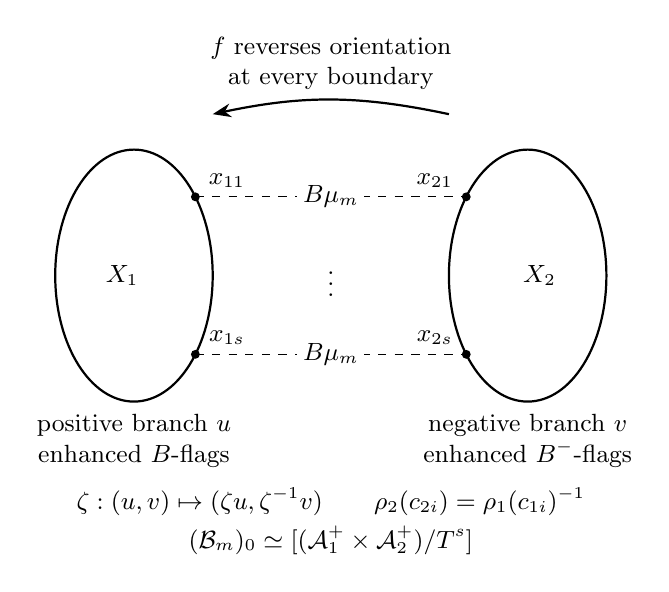
\begin{tikzpicture}[x=1cm,y=1cm,>=Stealth,font=\small]
 \draw[thick] (-2.5,0) ellipse (1.0 and 1.6);
 \draw[thick] (2.5,0) ellipse (1.0 and 1.6);
 \node at (-2.65,0) {$X_1$};
 \node at (2.65,0) {$X_2$};
 \foreach \yy/\ii in {1/1,-1/s} {
   \fill (-1.72,\yy) circle (1.6pt);
   \fill (1.72,\yy) circle (1.6pt);
   \draw[dashed] (-1.72,\yy)--(1.72,\yy);
   \node[above] at (-1.32,\yy) {$x_{1\ii}$};
   \node[above] at (1.32,\yy) {$x_{2\ii}$};
   \node[fill=white,inner sep=2pt] at (0,\yy) {$B\mu_m$};
 }
 \node at (0,0) {$\vdots$};
 \node[align=center] at (-2.5,-2.1)
      {positive branch $u$\\enhanced $B$-flags};
 \node[align=center] at (2.5,-2.1)
      {negative branch $v$\\enhanced $B^-$-flags};
 \draw[->,thick] (1.5,2.05) to[bend right=12]
       node[above,align=center] {$f$ reverses orientation\\at every boundary}
       (-1.5,2.05);
 \node[align=center] at (0,-3.12)
      {$\zeta:(u,v)\mapsto(\zeta u,\zeta^{-1}v)$\qquad
       $\rho_2(c_{2i})=\rho_1(c_{1i})^{-1}$\\[3pt]
       $\displaystyle (\cB_m)_0\simeq
         [(\cA_1^+\times\cA_2^+)/T^s]$};
\end{tikzpicture}
\caption{Normalization and gluing at all $s$ nodes (schematically).
The ovals are the coarse curves of the normalized root stacks.
The dashed pairs are identified, not extra curve components.
For bundle types the gerbes have fixed order $m$ and each pair
contributes one frame-change torus to the displayed quotient.
For parameter covers at stage $r$, replace $m$ by $m_r$ and
$\rho_j$ by its finite quotient at that stage.  The inverse boundary actions
then agree on the gluing gerbe, because its common generator acts
oppositely on the two branch coordinates.}\label{con:gluing-figure}
\end{figure}

\begin{lemma}\label{con:parameter}
Put $K_1=\overline{\mathbb C((z))}$ and let $C_{K_1}$ be the smooth
geometric generic curve.  There is a continuous unramified parameter
$\rho_{K_1}$ on $C_{K_1}$ with the same compact image as $\rho_1$.
Its lattice reductions specialize on $U_1\sqcup U_2$ to those of
$\rho_1$ and $\rho_2$, with the tensor compatibilities of
Proposition~\ref{found:hecke-specialization}.
\end{lemma}

\begin{proof}
Let $H=\rho_1(\pi_1^{\et}(U_1))\subset\Gd(L')$ be the compact
image, for a finite coefficient field $L'$.  Choose a cofinal
decreasing sequence of open normal subgroups $H_r$ and put
$Q_r=H/H_r$.  One obtains such a sequence from congruence kernels
of an $H$-stable lattice in a faithful representation.  Both $U_j$
carry connected $Q_r$-torsors.  Choose indices $m_r$ divisible by
the fixed $m$ and by the orders of all their boundary images, with
$m_r\mid m_{r+1}$.

By the root-stack description of tame covers
\cite[Proposition~A.10]{LieblichOlsson}, the torsors extend to finite
\'etale torsors on the normalization of $C(m_r)_0$.  At each pair
of gerbes their actions agree: the node identifies a positive
generator on the first branch with a negative generator on the
second, and \eqref{con:boundary-inversion} cancels that inversion.
Reduce the chosen boundary-fiber identifications modulo $H_r$ to
identify these restrictions.  They are compatible at every level of
the tower.  The torsors glue to a finite \'etale $Q_r$-torsor
$Y_{r,0}$ on $C(m_r)_0$.  Locally this is nodal gluing of finite
\'etale algebras with identified fibers: on the completed branch
discs the covers are constant, with the same $\mu_{m_r}$-action at
the origin, so their gluing is constant on the nodal cover and
descends equivariantly.  This also proves compatibility under the
power maps of the twisted models.

Proper henselian invariance of finite \'etale covers lifts $Y_{r,0}$
to a torsor $Y_r$ over $C(m_r)$
\cite[Theorem~4.5]{Rydh}.  Its hypotheses hold because the models
are proper with finite diagonal over complete henselian traits.
Full faithfulness lifts the group actions, transition maps after
pullback to divisible models, and all relations between them.
All generic fibers become $C_{K_1}$.  Choose a base section
specializing in $U_1$ and compatible points of the torsor fibers
above it; finite \'etale covers of this strictly henselian section
are constant.  The tower therefore gives a continuous homomorphism
\begin{equation}\label{con:generic-homomorphism}
 \rho_{K_1}:\pi_1^{\et}(C_{K_1})\longrightarrow
                      \varprojlim_r Q_r=H.
\end{equation}

We check its image.  Each $Y_{r,0}$ is connected, since its two
normalization torsors are connected and are glued along nonempty
fibers.  The total torsor $Y_r$ is proper and flat with reduced
geometric fibers.  Its tame coarse space is flat as well: locally
its coordinate ring is the $\mu_{m_r}$-invariant direct summand of an
$R_{m_r}$-flat ring, and invariant formation commutes with base change.
The connected reduced proper special fiber has
$H^0(\mathcal O)=\mathbb C$.  Semicontinuity, applied to the coarse
space, gives $h^0(Y_{r,K_1},\mathcal O)=1$, so the geometric generic
torsor is connected.  Thus \eqref{con:generic-homomorphism} surjects
onto every $Q_r$.  Its image is compact and therefore closed in $H$;
surjectivity to this cofinal system makes it all of $H$.  In
particular the parameter remains Zariski dense.

For an algebraic representation of $\Gd$, enlarge its finite
coefficient field if necessary and choose an $H$-stable lattice.
Each finite reduction factors through some $Q_r$.  Its lifted
torsor supplies a lisse extension over the smooth leg locus after
the corresponding finite trait extension, with the specified
special reductions on both components.  All twisted models agree
away from the nodes.  The tower thus gives the required tensor
compatibilities; maps between lattices are compared after clearing
denominators.  As allowed in
Proposition~\ref{found:hecke-specialization}, different reductions
may require different finite trait extensions.
\end{proof}

\subsection{A nonzero specialization and descent}

Lemma~\ref{con:unramified} now supplies a nonzero locally bounded
constructible eigencomplex $F$ on $\Bun_G(C_{K_1})$ with parameter
$\rho_{K_1}$.  Take its geometric nearby cycles on the fixed model
$\cB_m$.  Propositions~\ref{found:nearby} and
\ref{found:hecke-specialization}, with the geometry and lattice
extensions just verified, give a locally bounded constructible
eigencomplex $\Psi F$ on $(\cB_m)_0$, for legs on both $U_1$ and
$U_2$.  To use it we must prove nonvanishing on precisely this
prescribed-type fiber.

Choose a point of the product in \eqref{con:special-quotient} and
lift its image to a reference bundle $P_0$ over $R_m$.  This is
possible by smoothness of $\cB_m$: lift a point in a smooth chart
over the henselian trait.  Choose also a section $y$ of the smooth
scheme locus, disjoint from the nodes.  Since $F$ is nonzero, some
$K_1$-valued bundle $P$ has nonzero stalk.  Both $P$ and $(P_0)_{K_1}$
are trivial on the affine curve $C_{K_1}\setminus\{y_{K_1}\}$.
Indeed, a rank-$n$ projective module over a Dedekind domain is the
sum of a free rank-$(n-1)$ module and its determinant; an
$\mathrm{SL}_n$-bundle has trivial determinant, and its frame can be
adjusted to respect the chosen determinant trivialization.

An isomorphism off $y_{K_1}$ exhibits $P$ as a modification of
$(P_0)_{K_1}$ in a finite Schubert bound.  Its point is defined over
a finite extension of the trait's fraction field.  Properness of
the bounded Hecke space over the fixed input $P_0$ and leg $y$
extends this modification over the resulting trait.  Its output
still has the prescribed types, because the modification is away
from all nodes.  Lift this section to a finite-type smooth chart
through its special value.  Its generic stalk is the chosen nonzero
stalk, so the closure of the generic nonzero-stalk locus on this
chart meets the special fiber.  Theorem~\ref{det:specialization}
therefore gives
\begin{equation}\label{con:nonzero-nearby}
                         \Psi F\ne0.
\end{equation}
Here finite extensions cause no change to geometric nearby cycles,
as in Proposition~\ref{found:nearby}.

Pull back $\Psi F$ ordinarily along the smooth surjection
$\cA_1^+\times\cA_2^+\to(\cB_m)_0$.  Its pullback is nonzero.
By local constructibility choose a $\mathbb C$-valued point
$(a_1,a_2)$ with nonzero stalk and restrict to
$\cA_1^+\times\{a_2\}$.  This gives a nonzero locally bounded
constructible complex $F_1^+$ on $\cA_1^+$.  By
Lemma~\ref{con:quotient}, the first component's Hecke correspondences
are the base changes of those downstairs and act on the first
factor alone.  Proper base change on each bound makes both
pullbacks compatible with the full coherent Hecke system.  Thus
$F_1^+$ has eigenvalue $\sigma$.  These are ordinary pullbacks;
perversity will be obtained after descent.

\begin{proposition}\label{con:charzero}
Let $X/\mathbb C$ be a smooth projective connected curve of genus
at least two, with $s\geq2$ distinct marked points, divisor $D$ their
sum, and $G=\mathrm{SL}_n$.
Let $\sigma$ be a continuous dense $\Gd$-parameter on their
complement, defined over a finite coefficient extension, with
unipotent monodromy at every marking.  Then
$\Bun_{G,B,D}(X)$ carries a nonzero locally constructible perverse
geometric $E$-adic eigensheaf with eigenvalue $\sigma$, nilpotent
singular support, and the full coherent Hecke system in relative
Satake normalization.
\end{proposition}

\begin{proof}
The construction gives $F_1^+$ on the enhanced stack for $X$.
Proposition~\ref{desc:ordinary} applies because the parameter is
dense and each boundary monodromy is unipotent, and gives a nonzero
perverse eigenobject on the ordinary-flag stack.  Its singular
support lies in the required cone by Theorem~\ref{det:field}.
No regularity of any local nilpotent is used.
\end{proof}

\section{Lifting the parameter and specializing to characteristic
\texorpdfstring{$p$}{p}}\label{lift:section}

We return to the curve and parameter of Theorem~\ref{intro:main}.
The remaining step is to lift the marked curve and its parameter to
characteristic zero, apply Proposition~\ref{con:charzero}, and
specialize the resulting perverse eigensheaf.  We retain the full
inertia homomorphisms in the lift, including when some $N_i$ vanish.

Let $R=W(k)$.  This is an excellent complete strictly henselian
discrete valuation ring, and $\ell$ is invertible in $R$.  There is
a smooth projective lift with disjoint marked sections
\[
 (\mathscr X,\mathfrak x_1,\ldots,\mathfrak x_s)
                         \longrightarrow\Spec R
\]
of $(X,x_1,\ldots,x_s)$.  Indeed, the obstruction group for the
marked curve is $H^2(X,T_X(-D))=0$; an ample line bundle also lifts,
and formal algebraization gives the projective family.  Use the
split models of $G$ and $B$ over $R$, and put
\[
 \mathscr D=\sum_i\mathfrak x_i,\qquad
 \mathscr U=\mathscr X\setminus|\mathscr D|,\qquad
 K_0=\overline{\operatorname{Frac}(R)}.
\]

\begin{lemma}\label{lift:parameter}
The parameter $\rho$ lifts to a continuous parameter
$\rho_{K_0}:\pi_1^{\et}(\mathscr U_{K_0})\to\Gd(L)$ with the same
compact image.  After compatible choices of boundary fibers and
prime-to-$p$ roots of unity, its full inertia homomorphism at
$\mathfrak x_i$ is
\begin{equation}\label{lift:inertia}
 \rho_{K_0}(\gamma)=\exp\bigl(t_{\ell,i}(\gamma)N_i\bigr).
\end{equation}
In particular every other prime factor of characteristic-zero
inertia acts trivially.  Its lattice reductions extend lisse over
$\mathscr U$ and specialize to those of $\rho$, with the tensor
compatibilities of Proposition~\ref{found:hecke-specialization}.
\end{lemma}

\begin{proof}
We use the finite-cover lifting argument of
\cite[Section~8.5, Lemma~8.4]{CT}, applied at all the disjoint
markings.  Let $H=\rho(\pi_1^{\et}(U))$, choose a cofinal system
$Q_r=H/H_r$ as in Lemma~\ref{con:parameter}, and let $Y_r^\circ$
be the corresponding connected finite \'etale torsor on $U$.
At every marking its inertia image has $\ell$-power order, since
the given inertia homomorphism factors through $\mathbb Z_\ell$.
Choose $d_r=\ell^{e_r}$ divisible by all these orders at stage $r$,
with $d_r\mid d_{r+1}$.  The torsor extends to the proper root stack
\[
 X_r=X\bigl(\sqrt[d_r]{x_1},\ldots,\sqrt[d_r]{x_s}\bigr).
\]
This is the root-stack description of tame covers
\cite[Proposition~A.10]{LieblichOlsson}.  The corresponding relative
root stack
\[
 \mathscr X_r=
 \mathscr X\bigl(\sqrt[d_r]{\mathfrak x_1},\ldots,
                         \sqrt[d_r]{\mathfrak x_s}\bigr)
\]
is smooth, proper, and tame with finite diagonal over $R$, since
$d_r$ is invertible in $R$.

Proper henselian invariance lifts the finite \'etale torsors to
$\mathscr X_r$ \cite[Theorem~4.5]{Rydh}; full faithfulness lifts
their group actions, transition maps after pullback to divisible
root stacks, and all compatibility relations.  See also
\cite[Theorem~A.11 and Corollaries~A.12--A.13]{LieblichOlsson}.
Restricting to $\mathscr U$ and then to its geometric generic fiber,
and choosing compatible base points, produces
\[
 \rho_{K_0}:\pi_1^{\et}(\mathscr U_{K_0})\longrightarrow H.
\]
Only the root indices must be prime to $p$; the finite group orders
$|Q_r|$ need not be.

The special torsor on $X_r$ is connected: its inverse image of $U$
is dense and is the connected torsor $Y_r^\circ$.  It is smooth and
geometrically reduced.  The proper flat tame-coarse-space argument
in Lemma~\ref{con:parameter} gives connected geometric generic
root-stack torsors.  A smooth connected curve stack is irreducible;
removing the inverse images of the finitely many marked gerbes
therefore leaves it connected.  Thus $\rho_{K_0}$ surjects onto
every $Q_r$, and its compact image is all of $H$.  In particular
the lifted parameter is Zariski dense.

To determine inertia, trivialize the normal line of each marked
section over the strictly henselian trait.  Its root gerbes are
then $B\mu_{d_r}$, with compatible atlases as $r$ varies.
Restricting the lifted torsor to this gerbe and pulling to its atlas
gives a constant finite torsor together with its $\mu_{d_r}$-action.
Full faithfulness of lifting retains exactly the special-fiber
action.  Compatible prime-to-$p$ roots of unity identify the generic
and special generators.  One may choose the boundary frames
compatibly throughout the tower: the possible frames form an
inverse system of nonempty finite fibers with surjective transition
maps.  At every stage, generic inertia consequently
factors through $\mu_{d_r}$ and agrees with the original inertia map.
Passing to the inverse limit proves \eqref{lift:inertia} for the
whole inertia group.  In particular its $\mathbb Z_a(1)$ factor
acts trivially for every prime $a\ne\ell$, including $a=p$.
This records the full peripheral compatibility, rather than only
the conjugacy class of one monodromy element; compare
\cite[Lemma~3.5]{LieblichOlsson}.

Finally, each finite reduction of an $H$-stable lattice in an
algebraic representation factors through some $Q_r$.  The lifted
torsor restricted to $\mathscr U$ is lisse and has the required
special fiber.  Tensor products and maps between the resulting
systems come from the same tower, with denominators cleared when
comparing lattices.  This proves the asserted lattice extension
condition.
\end{proof}

We may identify $K_0$ abstractly with $\mathbb C$.  Indeed $k$ is
countable and $W(k)$ is a set of sequences in $k$, while it contains
$\mathbb Z_p$.  Its cardinality, and hence that of $K_0$, is the
continuum.  An uncountable algebraically closed characteristic-zero
field has transcendence degree equal to its cardinality, so $K_0$
and $\mathbb C$ are isomorphic.  This identification is only of the
geometric base fields; the adic topology of the coefficient field
and continuity of the parameter remain unchanged.

\begin{proof}[Proof of Theorem~\ref{intro:main}]\label{lift:main-proof}
By Lemma~\ref{lift:parameter} and Proposition~\ref{con:charzero},
the ordinary-flag bundle stack over $K_0$ has a nonzero locally
constructible perverse eigenobject $M_{K_0}$ with eigenvalue
$\rho_{K_0}$.  Put
\[
 \mathscr A=\Bun_{G,B,\mathscr D}(\mathscr X/R),\qquad
                  M=\Psi M_{K_0}\quad\text{on }\mathscr A_k=\cA.
\]
The stack $\mathscr A$ is smooth over $R$: the unlevelled bundle
stack is smooth by vanishing of the degree-two obstruction groups,
and its flag fibers are products of the smooth variety $G/B$.
Proposition~\ref{found:nearby} implies that $M$ is locally
constructible and perverse.  Thus for a smooth finite-type chart
$f:S\to\cA$ of relative dimension $d$, the complex $f^*M[d]$ is
bounded constructible and perverse.  These are geometric nearby
cycles, without taking inertia invariants.

The Hecke geometry on $\mathscr U$ is the split smooth-leg geometry
of Section~\ref{found:section}.  The lattice extensions in
Lemma~\ref{lift:parameter} and
Proposition~\ref{found:hecke-specialization} give
\begin{equation}\label{lift:final-eigenmaps}
 \Hecke_{I,(V_i)}(M)\simeq
 M\boxtimes\Bigl(\boxtimes_{i\in I}(V_i)_\rho\Bigr)
 \qquad\text{on }\cA\times U^I.
\end{equation}
This is the relative Satake normalization
$E[d_\lambda](d_\lambda/2)$, with no moving-leg shift.  The
isomorphisms are natural in all $V_i$ and retain the unit,
convolution, permutation, and fusion compatibilities on every
collision diagonal, since specialization transports the coherent
system itself.

It remains to show that $M$ is nonzero.  Local constructibility gives
a $K_0$-valued point $(P,(\beta_i))$ of the geometric generic bundle
stack at which $M_{K_0}$ has nonzero stalk.  Choose a reference
bundle $P_0$ on $\mathscr X$, for example the trivial bundle.
A point of $U$ lifts to a section $y$ of $\mathscr U$ by
smoothness and henselianity.  On the affine curve
$\mathscr X_{K_0}\setminus\{y_{K_0}\}$, both $P$ and $(P_0)_{K_0}$
are trivial by the determinant argument used in
Section~\ref{con:section}.  Hence $P$ is a modification of
$(P_0)_{K_0}$ at $y_{K_0}$ in some finite Schubert bound.  After
a finite trait extension defining the data, properness of the
bounded unlevelled Hecke space extends the modification and thus
the bundle.  Each flag $\beta_i$ then extends by properness of the
associated $G/B$-bundle over the marked section.  We have extended
the original point to the relative ordinary-flag stack.

Lift this section to a finite-type smooth chart through its special
value, after a further henselian lift if necessary.  Its generic
stalk is still nonzero, so the closure of the generic nonzero-stalk
locus meets the special fiber on that chart.  Theorem~\ref{det:specialization}
forces $\Psi M_{K_0}\ne0$.  Its hypotheses hold by the Hecke
geometry above, the lattice extensions of
Lemma~\ref{lift:parameter}, and the special-fiber geometry of
Section~\ref{geom:section}.  Geometric nearby cycles are unchanged
by the finite trait extensions used in this argument.

Finally, Theorem~\ref{det:field}, applied to
\eqref{lift:final-eigenmaps}, gives $\SS(M)\subset\Lambda$ on every
smooth chart.  At ordinary flag level,
Definition~\ref{geom:cone} and its cotangent description identify
this with the cone of generically nilpotent Higgs fields
\[
 \phi\in H^0\bigl(X,\ad(P)\otimes\omega_X(D)\bigr),\qquad
 \Res_{x_i}\phi\in\Lie R_u(B_{\beta_i})\quad(1\leq i\leq s).
\]
The condition $p>n$ gives precisely the characteristic hypotheses
used in that geometry and detection.  The nonzero sheaf $M$ has
all the asserted properties.  Every parameter and sheaf used in
the construction is geometric; no Frobenius structure is required.
\end{proof}

\begin{thebibliography}{99}
\raggedright

\bibitem{AGKRRV}
D. Arinkin, D. Gaitsgory, D. Kazhdan, S. Raskin, N. Rozenblyum, and
Y. Varshavsky, \emph{The stack of local systems with restricted variation
and geometric Langlands theory with nilpotent singular support},
preprint, 2020, revised 2022,
\href{https://arxiv.org/abs/2010.01906v2}{arXiv:2010.01906v2}.

\bibitem{AB}
S. Arkhipov and R. Bezrukavnikov, \emph{Perverse sheaves on affine flags
and Langlands dual group}, with an appendix by R. Bezrukavnikov and
I. Mirkovi\'c, Israel J. Math. \textbf{170} (2009), 135--183.
\href{https://doi.org/10.1007/s11856-009-0024-y}{doi:10.1007/s11856-009-0024-y}.

\bibitem{Barrett}
O. Barrett, \emph{The singular support of an $\ell$-adic sheaf},
Tunisian J. Math. \textbf{6} (2024), no.~4, 703--734.
\href{https://doi.org/10.2140/tunis.2024.6.703}{doi:10.2140/tunis.2024.6.703}.

\bibitem{Beilinson}
A. Beilinson, \emph{Constructible sheaves are holonomic},
Selecta Math. (N.S.) \textbf{22} (2016), no.~4, 1797--1819.
\href{https://doi.org/10.1007/s00029-016-0260-z}{doi:10.1007/s00029-016-0260-z}.

\bibitem{BD}
A. Beilinson and V. Drinfeld, \emph{Quantization of Hitchin's integrable
system and Hecke eigensheaves}, preprint.
\href{https://math.uchicago.edu/~drinfeld/langlands/QuantizationHitchin.pdf}{Authors' manuscript}.

\bibitem{DT}
G. Dhillon and J. Taylor, \emph{The universal monodromic
Arkhipov--Bezrukavnikov equivalence}, preprint, 2025,
\href{https://arxiv.org/abs/2501.14156v1}{arXiv:2501.14156v1}.

\bibitem{DTLocal}
G. Dhillon and J. Taylor, \emph{Tame local Betti geometric Langlands},
preprint, 2025,
\href{https://arxiv.org/abs/2501.14157v1}{arXiv:2501.14157v1}.

\bibitem{Drinfeld}
V. G. Drinfeld, \emph{Two-dimensional $\ell$-adic representations of the
fundamental group of a curve over a finite field and automorphic forms
on $\GL(2)$}, Amer. J. Math. \textbf{105} (1983), no.~1, 85--114.
\href{https://doi.org/10.2307/2374382}{doi:10.2307/2374382}.

\bibitem{Faergeman}
J. F{\ae}rgeman, \emph{Motivic realization of rigid $G$-local systems on
curves and tamely ramified geometric Langlands}, preprint, 2024,
\href{https://arxiv.org/abs/2405.18268v2}{arXiv:2405.18268v2}.

\bibitem{Faltings}
G. Faltings, \emph{Stable $G$-bundles and projective connections},
J. Algebraic Geom. \textbf{2} (1993), no.~3, 507--568.

\bibitem{FGV}
E. Frenkel, D. Gaitsgory, and K. Vilonen, \emph{On the geometric
Langlands conjecture}, J. Amer. Math. Soc. \textbf{15} (2002), no.~2,
367--417.
\href{https://doi.org/10.1090/S0894-0347-01-00388-5}{doi:10.1090/S0894-0347-01-00388-5}.

\bibitem{GaitsgoryCentral}
D. Gaitsgory, \emph{Construction of central elements in the affine
Hecke algebra via nearby cycles}, Invent. Math. \textbf{144} (2001),
no.~2, 253--280.
\href{https://doi.org/10.1007/s002220100122}{doi:10.1007/s002220100122}.

\bibitem{GaitsgoryVanishing}
D. Gaitsgory, \emph{On a vanishing conjecture appearing in the geometric
Langlands correspondence}, Ann. of Math. (2) \textbf{160} (2004), no.~2,
617--682.
\href{https://doi.org/10.4007/annals.2004.160.617}{doi:10.4007/annals.2004.160.617}.

\bibitem{GLCI}
D. Gaitsgory and S. Raskin, \emph{Proof of the geometric Langlands
conjecture I: construction of the functor}, preprint, 2024,
revised 2025,
\href{https://arxiv.org/abs/2405.03599v3}{arXiv:2405.03599v3}.

\bibitem{GLCV}
D. Gaitsgory and S. Raskin, \emph{Proof of the geometric Langlands
conjecture V: the multiplicity one theorem}, preprint, 2024,
revised 2026,
\href{https://arxiv.org/abs/2409.09856v3}{arXiv:2409.09856v3}.

\bibitem{GR}
D. Gaitsgory and S. Raskin, \emph{Geometric Langlands in positive
characteristic from characteristic zero}, preprint, 2025,
\href{https://arxiv.org/abs/2508.02237v1}{arXiv:2508.02237v1}.

\bibitem{GinzburgNilpotent}
V. Ginzburg, \emph{The global nilpotent variety is Lagrangian},
Duke Math. J. \textbf{109} (2001), no.~3, 511--519.
\href{https://doi.org/10.1215/S0012-7094-01-10933-2}{doi:10.1215/S0012-7094-01-10933-2}.

\bibitem{HallRydh}
J. Hall and D. Rydh, \emph{Coherent Tannaka duality and algebraicity of
Hom-stacks}, Algebra Number Theory \textbf{13} (2019), no.~7, 1633--1675.
\href{https://doi.org/10.2140/ant.2019.13.1633}{doi:10.2140/ant.2019.13.1633}.

\bibitem{HS}
D. Hansen and P. Scholze, \emph{Relative perversity},
Commun. Amer. Math. Soc. \textbf{3} (2023), 631--668.
\href{https://doi.org/10.1090/cams/21}{doi:10.1090/cams/21}.

\bibitem{Laumon}
G. Laumon, \emph{Correspondance de Langlands g\'eom\'etrique pour les
corps de fonctions}, Duke Math. J. \textbf{54} (1987), no.~2, 309--359.
\href{https://doi.org/10.1215/S0012-7094-87-05418-4}{doi:10.1215/S0012-7094-87-05418-4}.

\bibitem{LaumonNilpotent}
G. Laumon, \emph{Un analogue global du c\^one nilpotent},
Duke Math. J. \textbf{57} (1988), no.~2, 647--671.
\href{https://doi.org/10.1215/S0012-7094-88-05729-8}{doi:10.1215/S0012-7094-88-05729-8}.

\bibitem{LieblichOlsson}
M. Lieblich and M. Olsson, \emph{Generators and relations for the
\'etale fundamental group}, Pure Appl. Math. Q. \textbf{6} (2010),
no.~1, 209--243.
\href{https://doi.org/10.4310/PAMQ.2010.v6.n1.a6}{doi:10.4310/PAMQ.2010.v6.n1.a6}.

\bibitem{MV}
I. Mirkovi\'c and K. Vilonen, \emph{Geometric Langlands duality and
representations of algebraic groups over commutative rings},
Ann. of Math. (2) \textbf{166} (2007), no.~1, 95--143.
\href{https://doi.org/10.4007/annals.2007.166.95}{doi:10.4007/annals.2007.166.95}.

\bibitem{NY}
D. Nadler and Z. Yun, \emph{Spectral action in Betti geometric
Langlands}, Israel J. Math. \textbf{232} (2019), 299--349.
\href{https://doi.org/10.1007/s11856-019-1871-9}{doi:10.1007/s11856-019-1871-9}.

\bibitem{NYGluing}
D. Nadler and Z. Yun, \emph{Automorphic gluing functor in Betti
geometric Langlands}, preprint, 2021, revised 2023,
\href{https://arxiv.org/abs/2105.12318v3}{arXiv:2105.12318v3}.

\bibitem{OlssonTwisted}
M. C. Olsson, \emph{(Log) twisted curves},
Compos. Math. \textbf{143} (2007), no.~2, 476--494.
\href{https://doi.org/10.1112/S0010437X06002442}{doi:10.1112/S0010437X06002442}.

\bibitem{CT}
OpenAI, \emph{Constructible tame Hecke eigensheaves in positive
characteristic}, OpenAI Math Release preprint
\href{https://github.com/openai/math/blob/main/preprints/Constructible-tame-Hecke-eigensheaves-in-positive-characteristic-October-5-2026/constructible-tame-hecke-eigensheaves-positive-characteristic.pdf}{OAI:Constructible-tame-Hecke-eigensheaves-in-positive-characteristic-October-5-2026},
2026.

\bibitem{Rydh}
D. Rydh, \emph{Compactification of stacks and extending stackiness
across the boundary}, preprint, September~16, 2014.
\href{https://davidrydh.se/papers/compactification-survey20140916.pdf}{Author's manuscript}.

\bibitem{Shen}
S. Shen, \emph{Tamely ramified geometric Langlands correspondence in
positive characteristic}, Int. Math. Res. Not. IMRN \textbf{2024},
no.~7, 6176--6208.
\href{https://doi.org/10.1093/imrn/rnae005}{doi:10.1093/imrn/rnae005}.

\bibitem{Stacks}
The Stacks Project Authors, \emph{Stacks Project}, 2026.
\url{https://stacks.math.columbia.edu}.

\bibitem{UitDeBos}
N. uit de Bos, \emph{An explicit geometric Langlands correspondence for
the projective line minus four points}, Int. Math. Res. Not. IMRN
\textbf{2022}, no.~24, 19690--19746.
\href{https://doi.org/10.1093/imrn/rnab218}{doi:10.1093/imrn/rnab218}.

\end{thebibliography}

\end{document}
